%!TEX root=/home/ska124/Dropbox/Thesis/thes-full.tex
%% Copyright 1998 Pepe Kubon
%%
%% `thes-full.tex' --- the example thesis, FULL version, used
%%                     with  the `csthesis' package 
%% Use: latex thes-full to generate the DVI output, then 
%%      bibtex thes-full to generate the bibliography
%%      makeindex thes-full to get the index, and
%%      latex thes-full (2x) 
%%
%% You are allowed to distribute this file together with all files
%% mentioned in READ.ME.
%%
%% You are not allowed to modify its contents.
%%

\documentclass[11pt]{report}
%\documentclass[11pt,twoside]{report}%% for two-sided printing
\usepackage{pdfpages} 
\usepackage{anysize,fancyhdr,graphics}
\usepackage{csthesis}
\usepackage{makeidx}  %%% standard INDEX
\usepackage{booktabs}
\usepackage{tikz}
\usepackage{comment}
\usetikzlibrary{arrows}

\usepackage[titletoc]{appendix}%%Ensure word appendix appears in toc
\usepackage{algorithmic}
\usepackage{algorithm}
%% Custom Packages 

\usepackage{subfig,graphicx}
\usepackage{array}
\usepackage{enumitem}
\usepackage{listings}
\newcommand{\alert}[1]{{\textcolor{blue}{ALRT: #1}}}
\makeindex  

%%% The following code demonstrates the ``other list'' facility. A new
%%% command \otherlist is defined for the List of Programs. Programs
%%% are defined as floating environments of type 3 (1 is used for figures,
%%% 2 for tables) and the information about them is stored in an
%%% auxiliary file with .lop extension. You can use this method to
%%% define several types of ``other lists,'' but in that case you'll
%%% need to add appropriate code to \lists in the csthesis.sty
%%% package.
%%% Note: It's better to move this code into your own mythesis.sty
%%% package. If you do that, you should get rid of the \makeatletter,
%%% \makeatother commands.
\makeatletter
\newcommand\otherlist{%
    \addcontentsline{toc}{chapter}{\otherlistname}
    \if@twocolumn
      \@restonecoltrue\onecolumn
    \else
      \@restonecolfalse
    \fi
    \chapter*{\otherlistname
      \@mkboth{\MakeUppercase\otherlistname}%
              {\MakeUppercase\otherlistname}}%
    \@starttoc{lop}%
    \if@restonecol\twocolumn\fi
    }
\newcommand*\l@program{\@dottedtocline{1}{1.5em}{2.3em}}
\newcommand\otherlistname{List of Programs}
\newcommand\programname{Program}
\newcounter{program}[chapter]
\renewcommand\theprogram{\thechapter.\@arabic\c@program}
\def\fps@program{tbp}
\def\ftype@program{3}
\def\ext@program{lop}
\def\fnum@program{\programname~\theprogram}


%%%%%%%%%%%%%%%%%%%%%%%%%%%%%%%%%%%%%%%%%%%%%%%%%%%%%%%%%%%%%%%%%%%%%%
% mls: \code{...} command.
% Like \verb|...| but with braces, and not so fragile.
%
% Give me back the <, >, and _ characters in chosen modes
% unfortunately, this hack does not work when the <, >, or _ is embedded
% in another command.  In such circumstances use $<$, $>$, and \_
%
\makeatletter
\def\real@ltgtus{%
    \catcode`<=\active
    \catcode`>=\active
    \catcode`\_=\active
}
{\real@ltgtus
    \gdef<{\futurelet\@let@token\less@than}%
    \gdef>{\futurelet\@let@token\greater@than}%
    \gdef_{\underscore}%
}
% modify \textunderscore (standard LaTeX macro) to print as the _
% character in \tt font; as an appropriate rule in other fonts.
\renewcommand{\textunderscore}{\ifdim\fontdimen4\font=0pt\string_\else
    \leavevmode\kern.06em\vbox{\hrule width0.3em}\fi}
% \underscore is subscript in math mode, textunderscore otherwise
\DeclareRobustCommand{\underscore}{\ifmmode\sb\else\textunderscore\fi}
% similarly, create backslash, lessthan, and greaterthan macros that use
% the proper font:
\def\bs{\ifdim\fontdimen4\font=0pt\char92\relax\else
    \leavevmode$\backslash$\fi}
\newcommand{\less@than}{\ifdim\fontdimen4\font=0pt\string<\else
    \leavevmode\mathhexbox13C\fi}
\newcommand{\greater@than}{\ifdim\fontdimen4\font=0pt\string>\else
    \leavevmode\mathhexbox13E\fi}

% \code prints its argument in fixed-width font.
% There are no special characters in a code command, other than braces
% and backslash.
% It's similar to \verb, except that it's delimited normally (with
% braces).
\def\verythinspace{\kern .05em }
\DeclareRobustCommand{\code}{\begingroup
    \frenchspacing
    \real@ltgtus
    \@makeother\$\@makeother\&\@makeother\#%
    \@makeother\^\@makeother\%\@makeother\~%
    \@code}
\let\codefont\tt
\def\@code#1{\strut\verythinspace{\codefont
    #1}\verythinspace\strut\endgroup}
% For some reason I don't understand, escaped curly braces don't work
% right in \code commands.  Use the following instead:
\def\ttlb{{\tt\char123}}
\def\ttrb{{\tt\char125}}
\def\ttcaret{{\tt\char94}}
\def\tttilde{{\tt\char126}}
\makeatother
%%%%%%%%%%%%%%%%%%%%%%%%%%%%%%%%%%%%%%%%%%%%%%%%%%%%%%%%%%%%%%%%%%%%%%

%% Spots --- The round black magic blob

\def\spot#1{\begin{picture}(10,10)(-5,-4)%                                      
    \put(1,0){\circle*{10}}\put(-1,-3){\textcolor{white}{#1}}\end{picture}}

\def\bigspot#1{\begin{picture}(15,15)(-5,-5)%                                   
    \put(2,0){\circle*{15}}\put(-1,-3){\textbf{\textcolor{white}{#1}}}\end{picture}}



\newenvironment{program}
               {\@float{program}}
               {\end@float}
\newenvironment{program*}
               {\@dblfloat{program}}
               {\end@dblfloat}
\makeatother
%%% end of ``other list'' code
%\bibliography{thes-both.bib}
\begin{document}
\setlength{\pdfpagewidth}{8.5in}
\setlength{\pdfpageheight}{11in}
%%% set switches
%\contentspagefalse  
\figurespagetrue
\tablespagetrue
\dedicationpagetrue
\quotationpagetrue
% \otherlistpagetrue

%%% front matter 
%!TEX root=/home/ska124/Dropbox/Thesis/thes-full.tex
%% Copyright 1998 Pepe Kubon
%%
%% `titapp.tex' --- title and approval for thes-full.tex, thes-short-tex from
%%                  the `csthesis' bundle
%%
%% You are allowed to distribute this file together with all files
%% mentioned in READ.ME.
%%
%% You are not allowed to modify its contents.
%%

%%%%%%%%%%%%%%%%%%%%%%%%%%%%%%%%%%%%%%%%%%%%%
%
%   Title and approval pages
%
%%%%%%%%%%%%%%%%%%%%%%%%%%%%%%%%%%%%%%%%%%%%%

%%% title page

\title{Real-world use of pivot languages to translate low-resource languages}
\author{Rohit Dholakia}
\qualification{B.Tech, SASTRA University, 2010}
%\qualification{M.Xyf., Even Better University, 1994}
\submitdate{Spring 2014}
\copyrightyear{2014}

%%% approval page

\chair{Dr.~Ramesh Krishnamurthi} 
\signatory{Dr.~Anoop Sarkar, Senior Supervisor \\
        Associate Professor, Computing Science, \\ 
        Simon Fraser University \\ 
        }
\signatory{Prof.~Fred Popowich, Supervisor \\
        Professor, Computing Science, \\ 
        Simon Fraser University \\ 
        }
\signatory{Dr.~Greg Mori, Examiner \\
         Associate Professor, Computing Science, \\ 
        Simon Fraser University \\ 
        }
%%% generating title and approval pages 
\beforepreface

 %% title, approval

%% Partial Copyright License (PCL)
\newpage 			
\addcontentsline{toc}{chapter}{Partial Copyright License}
\mbox{}
\makeatletter
\AddToShipoutPictureBG*{
            \setlength{\@tempdimc}{.06\paperheight}
            \setlength{\unitlength}{1pt}
           \put(\strip@pt\@tempdimb,\strip@pt\@tempdimc){
	\includegraphics{PCL_Declaration_2011.pdf}
	} 
} 
\makeatother
\newpage

%!TEX root=/home/ska124/Dropbox/Thesis/thes-full.tex
%% Copyright 1998 Pepe Kubon
%%
%% `abstract.tex' --- abstract for thes-full.tex, thes-short-tex from
%%                    the `csthesis' bundle
%%
%% You are allowed to distribute this file together with all files
%% mentioned in READ.ME.
%%
%% You are not allowed to modify its contents.
%%

%%%%%%%%%%%%%%%%%%%%%%%%%%%%%%%%%%%%%%%%%%%%%%%%%
%
%       Abstract 
%
%%%%%%%%%%%%%%%%%%%%%%%%%%%%%%%%%%%%%%%%%%%%%%%%

\prefacesection{Abstract}

Triangulation refers to the use of a pivot language when translating from a source language to a target language. Previous research in triangulation has only focused on large corpora in the same domain.  This thesis conducts the first in-depth study on the use of triangulation for four real low-resource languages with realistic data settings, Mawukakan and Maninkakan, Haitian Kreyol and Malagasy, where fluent translations using statistical machine translation are difficult to obtain due to limited amounts of training data in the source-target language pair. We compare and contrast several design choices one needs to consider when using triangulation. We observe that triangulation via French improves translations significantly for Mawukakan and Maninkakan, two languages spoken in West Africa with no writing tradition. We also improve translations for real-world short messages sent in the aftermath of the Haiti earthquake in 2010 and news articles in Malagasy. This is the first in-depth study on triangulation for these four low-resource languages.

As part of the dissertation, we build the first effective translation system for three of these languages. We improve translation quality by injecting more data via pivot languages and show that in realistic data settings carefully considering triangulation design options is important. Furthermore, in all four languages since the low-resource language pair and pivot language pair data typically come from very different domains, we use insights from domain adaptation to fine-tune the weighted mixture of direct and pivot based phrase pairs to significantly improve translation quality. 





 %% abstract
%!TEX root=/home/ska124/Dropbox/Thesis/thes-full.tex
%% Copyright 1998 Pepe Kubon
%%
%% `dedquot.tex' --- dedication and quotation for thes-full.tex from
%%                   the `csthesis' bundle
%%
%% You are allowed to distribute this file together with all files
%% mentioned in READ.ME.
%%
%% You are not allowed to modify its contents.
%%

%%%%%%%%%%%%%%%%%%%%%%%%%%%%%%%%%%%%%%%%%%%%%
%
%   Dedication/Quotation pages
%
%%%%%%%%%%%%%%%%%%%%%%%%%%%%%%%%%%%%%%%%%%%%%

\dedication{To Mom}
\thesquot{%
``How I wish, how I wish you were here''\\[5pt]%
--- Wish you were here, \textsc{Pink Floyd}, 1975%
}

%%% generate pages

\dedicquotation















 %% dedication and quotation, if any 
%!TEX root=/home/ska124/Dropbox/Thesis/thes-full.tex
%% Copyright 1998 Pepe Kubon
%%
%% `ack.tex' --- aknowledgments for thes-full.tex, thes-short-tex from
%%               the `csthesis' bundle
%%
%% You are allowed to distribute this file together with all files
%% mentioned in READ.ME.
%%
%% You are not allowed to modify its contents.
%%

%%%%%%%%%%%%%%%%%%%%%%%%%%%%%%%%%%%%%%%%%%%
%
%       Acknowledgment 
%
%%%%%%%%%%%%%%%%%%%%%%%%%%%%%%%%%%%%%%%%%%

\prefacesection{Acknowledgements}

I am lucky to have a lot of people to thank. 

This dissertation would not be possible without my advisor, Dr. Anoop Sarkar. He let me choose a topic that got me excited, helped me through the lows and highs and his door is always open for guidance, advice and enlightment. It has been a joy to work with him. 

Without my Mom, I would have never dreamt of coming to Vancouver from a small town in rural India. She always told me to dream and work equally hard towards them. This dissertation and everything before and after is dedicated to her. 

To Sudha for standing by me all these years through thick and (quite a bit of) thin. Thanks for waiting and I hope you don't have to wait much longer. 

Thanks to my friends at SFU for humouring my sense of humour and being happy victims of my amateurish cooking skills. 










 























 %%  acknowledgments

%%%  generate contents, lists of figures, etc.
\lists

%% preface (foreword), if any
% %!TEX root=/home/ska124/Dropbox/Thesis/thes-full.tex
%% Copyright 1998 Pepe Kubon
%%
%% `preface.tex' --- preface for thes-full.tex from
%%                   the `csthesis' bundle
%%
%% You are allowed to distribute this file together with all files
%% mentioned in READ.ME.
%%
%% You are not allowed to modify its contents.
%%

%%%%%%%%%%%%%%%%%%%%%%%%%%%%%%%%%%%%%%%%%%%%%%%%%
%
%       Preface 
%
%%%%%%%%%%%%%%%%%%%%%%%%%%%%%%%%%%%%%%%%%%%%%%%%

\prefacesection{Preface}
Here go all the interesting reasons why you decided to write this thesis.

 

%%% prepare main section
\beforetext

%%% main matter - chapters
%!TEX root=/home/ska124/Dropbox/Thesis/thes-full.tex
%% Copyright 1998 Pepe Kubon
%%
%% `05-introduction.tex' --- 1st chapter for thes-full.tex, thes-short-tex from
%%                the `csthesis' bundle

%%%%%%%%%%%%%%%%%%%%%%%%%%%%%%%%%%%%%%%%%%%%%%%%%
%
%       Chapter 1 
%
%%%%%%%%%%%%%%%%%%%%%%%%%%%%%%%%%%%%%%%%%%%%%%%%

\chapter{Introduction}
\label{sec:introduction}

\section{Why study Low-Resource languages?}
\label{sec:low_resource}

Statistical Machine Translation(SMT) has enabled several languages like French, Spanish, Finnish and others to have publicly available translation systems which can translate from and into these languages. Google Translate has 81 languages you can translate from and to. In 2003, we had none ! 


Having said that, more than 90\% of the World languages do not have a publicly available SMT system. Moreover, most of them have not been studied in the SMT literature before. In Table~\ref{table:numberspeakers}, we observe that the major languages have way more number of speakers than the languages we study in this disseration. 
\begin{table*}
	\begin{tabular}{lr}
	\toprule
	Language & \#speakers \\
	\toprule
	French & 120M \\
	Spanish & 466M \\
	Mandarin Chinese & 1026M \\
	\midrule
	Haitian Kreyol & 12M \\
	Malagasy & 18M \\
	Mawu & 2M \\
	Manin & 2M \\
	\bottomrule
	\end{tabular}
	\caption{Number of speakers for Major and low-resource languages}
	\label{table:numberspeakers}
	%\small
	%\centering
\end{table*}

Studying languages with insufficient resources throws up interesting and unique linguistic challenges.  Providing a solution for the challenges takes us a little closer towards the quest for a universal translator. For instance, Malagasy has influence from French and Arabic. While there are some loan words from French, the numbers are written right-to-left like Arabic, while also having some vocabulary overlap with Bantu. Diacritics are used but only in certain circumstances. On the other hand, Mawukakan and Maninkakan show a more frequent usage of diacritics. But the accent can be different depending on the placement of the word. Haitian Kreyol is a French-based Creole but does not share any vocabulary with Parisian French. The influence is from 18th century French when Haiti was ruled by France. Haitian Kreyol became an official language only in 1961. Like is typical of Creoles, the morphology is not very rich but because the language is still undergoing changes, its not yet standardized. In the training corpus, there are a few English words that can be spelt 5 or 6 different ways.

\section{Phrase-based SMT Pipeline}
\label{sec:generic_pipelin}
To the interested reader, we refer to the comprehensive and readable SMT survey~\cite{Lopez07asurvey}. Below, we discuss the pipeline for phrase-based SMT~\cite{Koehn:03} which has been used for all the experiments in the dissertation, and discuss how a low-resource language pair raises question at each stage. 

SMT uses data-driven models to translate sentences in a source language to a given target language. Given a parallel corpus between \emph{s} and \emph{t}, a phrase-based SMT system has a generic pipeline that looks as described in Algorithm~\ref{algo:pbsmt}. 

\begin{algorithm}
\small
%\centering
\caption{Building a phrase-based system}
\label{algo:pbsmt}
\textbf{Input}: Parallel corpus between \emph{s} and \emph{t} \\
\textbf{Output}: A translation model ``tm'' 
\begin{algorithmic}[l]
	%\STATE{\textbf{Clean:}Pre-process both sides of the corpus} \label{aline:preprocess}
	\STATE{\textbf{Alignments: }Learn bi-directional alignments} \label{aline:alignments}
	\STATE{\textbf{Extraction: }Extract phrase pairs from alignments and compute likelihoods for each translation pair} \label{aline:scores}
	\STATE{\textbf{Tuning: }Set weights for features by maximizing BLEU score on a development set using MERT} \label{aline:MERT}
	\STATE{\textbf{Decoding: }Using language model and translation model, translate test sentences} \label{aline:decoding}
\end{algorithmic}
\end{algorithm}

The reason its called phrase-based SMT is because the base unit of translation are \emph{phrases}. The phrases need not be linguistically motivated. Phrases in this context means a continuous group of words. In this dissertation, we only use phrase-based SMT for all the experiments but there are others in the literature.~\cite{Chiang:07,Michel:04}

Each step of Algorithm~\ref{algo:pbsmt} outlined above raises questions when faced with a low-resource language pair. Low-resource languages are those with insufficient resources to use for Machine Translation into and/or from the language. To provide perspective, French has a corpus with $10^9$ parallel sentences with English. On the other hand, the language with the highest amount of data in this dissertation is Haitian Kreyol, with 121K sentences. Out of those 121K, only 16\% are from the target domain, the sentences are noisy and with punctuation and spelling mistakes.


Lets consider each step and discuss the problems that come up. Given parallel data, the goal of the alignment models~\cite{Brown:1993,Vogel:1996} is to learn which word in source language \emph{s} translates to target language \emph{t} and assign a likelihood to the pair of words. The advanced alignment models use initial alignments from IBM Model 1. Model 1 starts with uniform initialization and uses Expectation Maximization~\cite{Dempster:77} to converge. Facing a corpus of a small size, the alignment models will end up making inferences that are not always true. They will place higher likelihood on pairs seen fewer number of times due to lack of more data. At the end of the alignment process, we will have two alignment files. The forward alignment file will say which words in the target language align to which words in the source language. The backward alignment file will say vice-versa. An entry from the backward and forward alignment files would look like shown in Table~\ref{table:example_fwd_backward}. The \emph{forward} line says that the target word ``a'' is aligned to nothing on the source side, while bit is aligned to enpe and everywhere is aligned to both tout and kote. The \emph{backward} line says the same thing but the target side is Haitian Kreyol. 

\begin{table*}
\small
\small
\begin{tabular}{lp{0.3\textwidth}p{0.5\textwidth}}
\toprule
direction & tgt & src \& alignment \\
\toprule
\emph{forward} & enpe tout kote & NULL ({ }) a ({ }) bit ({ 1 }) everywhere ({ 2 3 })  \\
\emph{backward} & a bit everywhere & NULL ({ }) enpe ({ 1 2 }) tout ({ }) kote ({ 3 }) \\
\bottomrule
\end{tabular}
\caption{Example of a forward and backward alignment}
\label{table:example_fwd_backward}
\end{table*}


The phrase extraction step(Line~\ref{aline:scores}) looks at alignments learnt from Line~\ref{aline:alignments} in both directions and determines which phrases can translate from one language to another using the intersection of the alignments. There are several ways of considering the intersection in the literature, but we consider the approach outlined in~\cite{Koehn:03}. Essentially, after the intersection, points are added if they are in the union of the bi-directional alignments and connects a previously unaligned word. This heuristic is known as \emph{grow-diag-final-and}. At the end of this step, we have a phrase table which has rules shown in Table~\ref{table:example_rule} : 

\begin{table*}[ht]
\small
\small
\centering
\begin{tabular}{p{0.3\linewidth}p{0.2\linewidth}p{0.4\linewidth}}
\toprule
src & tgt & features \\
\toprule
! la situacion de haiti & concerned about the situation in haiti & 0.5 8.16237e-09 1 0.000483004 2.718 \\
\bottomrule
\end{tabular}
\caption{Example of a phrase pair in the Haitian Kreyol to English table}
\label{table:example_rule}
\end{table*}

The table~\ref{table:example_rule}  says that the source phrase \textbf{! la situacion de haiti ,} translate to the target phrase \textbf{concerned about the situation in haiti ,} with the feature values shown on the right. 

\begin{table*}
	\small
	\small
	%\centering
	\begin{tabular}{p{0.3\linewidth}p{0.6\linewidth}}
	\toprule
	Feature &  Explanation \\
	\toprule
	$p_{w}(f \mid e)$ & probability of seeing phrase ``f'' given ``e'' \\
	$p_{lex}(f \mid e)$ & lexical probability of seeing phrase ``f'' given ``e'' \\
	$p_{w}(e \mid f)$ & probability of seeing phrase ``e'' given ``f'' \\
	$p_{lex}(e \mid f)$ & lexical probability of seeing phrase ``e'' given ``f'' \\
   	phrase penalty & a constant value penalizing distortion \\
	\bottomrule
	\end{tabular}
	\caption{Features of the phrase pairs, where ``f'' is foreign/source \& ``e'' is target/english}
	\label{table:features}
\end{table*}

The 5 features are mentioned in Table~\ref{table:features}. The two $p_{w}$ are the phrasal features, features that determine the likelihood of the source phrase translating to target and vice-versa. The phrasal translation likelihood is computed by using relative frequencies, as shown in equation~\eqref{eq:trans}.

\begin{equation} \label{eq:trans}
	p_{w}(f \mid e) = \frac{c(f, e)}{\mathlarger{\sum\limits_{\grave{f}}}c(\grave{f}, e)}
\end{equation}

The counts referred to in equation~\eqref{eq:trans} are obtained from the alignments. Note that the alignment models that were learnt on a small-sized corpus will cause some propagation of errors in the phrasal probabilities. 

The lexical features~\cite{Koehn:03} are actually computed as shown in equation~\eqref{eq:lex} : 

\begin{equation} \label{eq:lex}
	p_{lex}(f \mid e, a) = \prod\limits_{i=1}^{n} \frac{1}{\{j | (i,j) \in a\}}
	\mathlarger{\sum\limits_{\forall (i,j) \in a}} w(f_{i} \mid e_{j})
\end{equation}


The intuition behind having a pair of lexical features is to reward syntactic phrases while penalizing spurious ones. As shown in equation~\eqref{eq:lex}, the lexical probability is the product of the lexical alignment probabilities of the constituent words in the phrase table. Hence, if a longer source phrase aligns to an equally long target phrase, it can be penalized if the individual words are not aligned. 

Having learnt translation pairs with their respective features, we now want to know which features are better indicators of good translations and vice-versa. For weight learning, we use Minimum Error Rate Training. Before discussing MERT, its important to know about BLEU~\cite{Papineni:02}, Bilingual Evaluation Understudy. BLEU is the error metric used most often when comparing output translations with reference translations. BLEU compares an output translation with a reference translation according to equation~\eqref{eq:BLEU}

\begin{equation} \label{eq:BLEU}
	BLEU_{score} = BP. \sum\limits_{i=1}^n w_{i}p_{i}
\end{equation}

where $w_{i}$ is the weight to the n-gram while $p_{i}$ is the modified n-gram precision. 

Modified n-gram precision is a corpus-based count of the n-gram, which is modified to not count the co-occurences which are repeated in the same sentence. For instance, for an output translation, \begin{verbatim}the the the the the the the\end{verbatim} with a reference translation \begin{verbatim}the cat on a mat\end{verbatim}, the co-occurence of ``the'' is only counted once. And not 7 times. 

The modified precision explained above is defined as in equation~\eqref{eq:precision}

\begin{equation} \label{eq:precision}
	p_{n} = \frac{\mathlarger{\sum\limits_{c \in \{Candidates\}}} \mathlarger{\sum\limits_{n-gram \in c}Count_{clip}(n-gram)}}
			{\mathlarger{\sum\limits_{\acute{c} \in \{Candidates\}}} \mathlarger{\sum\limits_{n-gram\acute{} \in \acute{c}}Count(n-gram\acute{})}}
\end{equation}

where Candidates refers to the target set of sentences. 

Minimum Error Rate Training chooses weights for features that minimize BLEU score loss given a ``tuning'' set. A ``tuning'' set is a set of parallel sentences between source and target that is in the same domain as the test and of the same type. For instance, when trying to improve translations for Haitian Kreyol short messages, we have tuning and test in the same domain, SMS, although our training is 85:15 mix of OOD:SMS. Essentially, MERT takes translation pairs generated from a mixture of domains corpus and tunes the weights such that the translations are more like that target domain. In Haitian Kreyol, as our training rules have been extracted from a smaller corpora that has not been manually sentence-aligned, MERT is learning weights for features that have values which are not always true. This is why we re-tune our weights for the interpolated model after obtaining a translated table with scaled values from the much larger fr-en table. 

The goal of MERT is to find parameters $\lambda_{1}^{M}$ for M feature functions $h_{1}^{M}$ to minimize the minimum BLEU loss, where BLEU is the error count metric, given set of source sentences $F_{1}^{S}$ with reference translations $R_{1}^{S}$, each source sentence having n-best candidate translations $c_{1}^{n}$. 

\begin{equation} \label{eq:maximization_mert}
	\hat{e}(f_{s};\lambda_{1}^M) = \argmax_{e \in C} \mathlarger\sum\limits_{m=1}^{M} \lambda_{m}h_{m}(e \mid f_{s})
\end{equation}



The error count is shown in equation~\eqref{eq:errorcount}\footnote{The equations about line search in MERT are from Phillipp Koehn's textbook on SMT}

\begin{equation} \label{eq:errorcount}
	\lambda_{1}^{M} = \argmin_{\lambda_{1}^{m}} \mathlarger{\sum\limits_{s=1}^{S}E(r_{s}, \hat{e}(f_{s};\lambda_{1}^{m}))}
\end{equation}

The key to MERT is doing a line search along one feature while keeping the others constant. Lets assume a corpus of one line. In the first iteration of MERT, a \emph{n-best} list will be generated. These are the top-\emph{n} translations by the decoder by using the default weights for all the features. For a given sentence, the n-best list might look like shown in Table~\ref{table:nbest}. After this n-best list is generated, the task is to find the best translation for the given source sentence. Remember that each sentence has several features and MERT has to learn weights for each. The overall likelihood for the sentence is defined by equation~\eqref{eq:line_likelihood}. The best is defined by the sentence which minimizes the error(equation~\eqref{eq:mert_best}). 

\begin{equation} \label{eq:line_likelihood}
	p(x) = \exp\mathlarger{\sum_{i=1}^n}\lambda_{i}h_{i}(x)
\end{equation}

\begin{equation} \label{eq:mert_best}
	x_{best}(\lambda_{1}, ..., \lambda_{n}) = argmax_{x}\exp\sum_{i=1}^n \lambda_{i}h_{i}(x)
\end{equation}

At this point, MERT decides to do a line search. We can learn the best weight for one feature, say at index ``c'', by keeping all the other features constant. This is shown in equation~\eqref{eq:line}


\begin{equation} \label{eq:line}
	u(x) = \mathlarger{\sum_{i \neq c}\lambda_{i}h_{i}(x)}
\end{equation}

Now, the equation~\eqref{eq:mert_best} will look like equation~\eqref{eq:new_best}. 

\begin{equation} \label{eq:new_best}
	x_{best}(\lambda_{c}) = argmax_{x} \lambda_{c}h_{c}(x) + u(x)
\end{equation} 

Now, each translation in the n-best list is the line of an equation and the points at which the best $\lambda$ for this line will change is at the points where the line intersects. The best $\lambda$ can be found in the same way for all the lines in the tuning set and the one that minimizes BLEU loss over the whole corpus becomes the weight for this feature. 

The process outlined above explains both the good and bad about MERT. The good being that MERT works effectively around the fact that we have a scenario of minimizing BLEU loss, which is not smoothed and which is a corpus level error metric, inside an \emph{argmax} as in equation ~\eqref{eq:maximization_mert}. The bad is that MERT does not scale to many features. At each iteration, weights have to be learnt for all the features. After the iteration, the n-best list is regenerated to have the maximum number of entries, done to cover the hypothesis space as much as possible. To avoid local minima, in practice, MERT is started from not one but a few random points.



\begin{table*}
	\begin{tabular}{p{0.4\textwidth}p{0.6\textwidth}}
		\toprule
		src & n-best list \\
		\toprule
		\multirow{10}{*}{ki kote y ap bay manje ?}  & \\ 
		& how can i find help for my province of aquin . \\
		& how can i find help for my in aquin . \\
		& how can i find help for my part of aquin . \\
		& how can i find help for my province of aquin ? \\
		& how can i find help for in my province of aquin . \\
		& how can i find aid for in my province of aquin . \\
		& how can i find help for my part aquin . \\
		& how can i find help for my in aquin ?  \\
		& how can i find help for my country aquin . \\
		& how can i find help for my in aquin . \\
		\bottomrule
	\end{tabular}
	\caption{Example of a n-best list, where n $\leq$ 100}
	\label{table:nbest}
\end{table*}




Having obtained the weights and a language model on the target side, decoding refers to the process of finding the best translation for the source sentence as shown in equation~\eqref{eq:decoding}. 

\begin{equation} \label{eq:decoding}
	e_{best} = \argmax_{e} \mathlarger{\prod\limits_{i=1}^I} \phi(\hat{f}_{i} | \hat{e}_{i})p_{LM}(e)d(start_{i} - end_{i-1}-1)
\end{equation}


Phrase-based SMT has been used with great success before in the literature. But, as described above, the approach is quite data-driven and it is not clear how to achieve fluent translations with only a little parallel data.  

\section{Examples using triangulation}

The easiest way to get better translations is to have more data between the source and target languages. As the amount of data increases, the models will learn the correct alignments which leads to more meaningful translation rules with accurate feature values and thus, more fluent translations. But, it will require a lot of human effort and time to get more parallel data between the low-resource source and target language. The second easiest way is to improve tokenization for the source and/or target language. Better tokenization goes a long way in pre-processing the text correctly. But, what do we do when these two options are not available ? 

\newcommand{\mawuexample}[1]{\emph{$y\grave{a}ng\acute{a}l\acute{a}\grave{a}$ w$\acute{\varepsilon}\acute{\varepsilon}$ $\grave{a}$ $\grave{a}$ l$\acute{a}$kw$\acute{e}$ k$\acute{o}\acute{o}$ b$\acute{\varepsilon}$ m$\grave{a}$ .}}

\newcommand{\anothermawu}[1]{\emph{\textipa{\!d}y$\grave{e}$n\textipa{\textltailn}$\acute{o}$ l$\grave{a}$ $\acute{i}$ kw$\acute{ɔ}$l$\grave{ɔ}$ $\acute{à}n$ d$\grave{a}$$\grave{a}$ l$\grave{u}$ m$\grave{a}$ }}

%\anothermawu is test
\begin{table}
	\caption{Without and with triangulation}
	\footnotesize
	\small
	\begin{tabular}{p{0.35\textwidth}p{0.45\textwidth}p{0.2\textwidth}}
	\toprule
	src & translations & Explanation \\
	\toprule
	\multirow{3}{*}{\mawuexample} 
	& her father y$\grave{a}$̀ng$\acute{a}$́l$\acute{o}$́$\grave{o}$̀ has l$\grave{a}$́kw$\grave{e}$́ everything . & translation from the direct system 
	\\ \cmidrule(r){2-3}
	&  the disease her father is not in a position to everything . & translation from the interpolated system 
	\\ \cmidrule(r){2-3}
	&  \emph{the illness has rendered her father invalid .}  & the reference 
	\\  
	\midrule
	\midrule
	\multirow{3}{*}{\anothermawu} 
	&  the entrance of the child behind her back and let us go home . & translation from the direct system \\
	\cmidrule(r){2-3}
	&  the child behind her back and let us go home . & translation from the interpolated system \\
	\cmidrule(r){2-3}
	& \emph{take the baby in your back and let 's go home !} & reference translation \\
	\bottomrule
	\end{tabular}
	\\[3.5pt]
	{\centering \emph{Example using Mawukakan as src, top-\emph{n} as interpolated model, both examples from heldout}}
	\label{table:mawu_improvement}
\end{table}


In the Table~\ref{table:mawu_improvement}, we mention two sentences in Mawu from the heldout data. The direct translation is the output translation we obtain by only using the 3K training sentences we have. The interpolated output shown is the output after interpolating a triangulated model with the direct translation model. The reference translation is the best translation for that sentence. The word \emph{$y\grave{a}ng\acute{a}l\acute{a}\grave{a}$} and \emph{l$\acute{a}$kw$\acute{e}$} are out-of-vocabulary words for the direct system. Words that have no translations in the phrase table are out-of-vocabulary words. By using an English translation via the Europarl corpus, we translate all the source words in the interpolated table. In the second example, all the source words are known. But, we get a weird ``the entrance'' phrase in the beginning. What went wrong ? When we look deeper, we see that ``the entrance'' is one of the top translations for the word l$\grave{a}́$, out of 23 translations in the direct table. After triangulation and interpolating with the direct system, it has 1615 translations and ``the entrance'' is nowhere to be seen in the top translations. This is because some of the translations of l$\grave{a}́$ have common pivot phrases which end up making the translation model give lower value to the existing ones. These are just two examples of how triangulation can reduce OOVs while also improving translations for existing phrases. 


The approach of triangulation~\cite{Cohn:07,Utiyama:07,Nakov:12} aims to add translations for new source phrases while also improving translations for existing source phrases. Both the aims are contingent on the common pivot phrases betwen the source pivot and pivot target tables. New source phrase translations(like shown in Table~\ref{table:mawu_improvement}) can be added if one has the source phrase in a source pivot corpora that leads to a new target phrase in the pivot target corpus. In a low resource scenario, its important to achieve both aims with triangulation. Owing to less training data, the direct system has several out-of-vocabulary(OOV) words. We aim to reduce the number by using triangulation. At the same time, it is reasonable to assume that the source phrases we do have translations for are not always right, as seen in the second example on Table~\ref{table:mawu_improvement}. We put our trust in triangulation to improve existing translations. 

\section{Dissertation Outline}
\label{sec:outline}

In chapter~\ref{chap:triangulation}, we discuss triangulation and the constituent models. In chapter~\ref{chapter:reality}, we report results on four real low-resource languages. In chapter~\ref{chap:related_work}, we discuss prior work and also compare our results with another ``low-resource'' setting using Europarl data. We conclude in chapter~\ref{chap:conclusion}

\section{Contributions of this dissertation}
\label{sec:summary}
We conduct the first in-depth study of triangulation, the first using four real low-resource languages with realistic data settings. As part of the dissertation, we also build the first translation systems for three of the four languages. Our best Haitian Kreyol system outperform the best system from the Sixth Workshop on Machine Translation, 2011. 


\section{Experimental Setup}
\label{sec:setup}


Moses~\cite{Koehn:07} was used for all the experiments. Moses is a leading publicly-available, open source SMT system with a rich documentation and active contributors. 

To build our baseline systems, we followed the standard set of steps: generated bi-directional alignments using GIZA++ ~\cite{OchNey:03}, followed by phrase extraction using the \emph{--grow-diag-final-and} heuristic. The heuristic intersects the alignments in both directions and takes the longest alignment that is common. The decoder parameters were optimized using Minimum Error Rate Training ~\cite{Och:03} by minimizing BLEU~\cite{Papineni:02} loss on a development set. All scores reported are case-insensitive BLEU. All language models were generated using SRILM~\cite{Stolcke:02}.~\cite{Ken:11} was used for language model scoring when decoding. SRILM is a language modeling toolkit for generating language models covering several smoothing and interpolation models. KenLM enables fast lookups in large language models by using efficient data structures.   
%!TEX root=/Users/rohitdholakia/Work/Thesis-Work/Thesis/thes-full.tex
%%%%%%%%%%%%%%%%%%%%%%%%%%%%%%%%%%%%%%%%%%%%%%%%%%%%
%
%     Chapter 3   
%
%%%%%%%%%%%%%%%%%%%%%%%%%%%%%%%%%%%%%%%%%%%%%%%%%

\chapter{Baselines}
\label{chap:baselines}

\section{Haitian-Creole}

\subsection{What is Haitian-Creole?}
	
	Creoles are languages that are a mixture of two or more languages. In general, there is a dominant language, which is the \emph{superstratum} and the other language is \emph{substratum}. Haitian-Creole is a French-based Creole, making French the superstratum language, and Fongbe, a West African language, is the substratum language. Superstratum is a language that is spoken by a small but powerful community ( like French in case of Haitian-Creole) and substratum is what is spoken by majority but common population. A creole comes about when the majority need to speak with the minority. So you get influences from both the classes~\cite{Claire:98}. Typically, the superstratum influences the grammar while the vocabulary has large influences from the substratum. This is observed in Haitian-Creole which has the same subject-verb-object behaviour as French, but the words in Haitian-Creole are different from French. Part of the reason behind the different vocabularies is that the French part of Haitian-Creole is not the Parisian French spoken and written today. Haitian-Creole has influences from 18th Century French, thus having words that might mean the same thing albeit spelt differently. There are several other instances of Creole in existence today, e.g, a form of French Creole is spoken in Quebec, Mauritian Creole is also a French-based Creole. Haitian-Creole has been in existence since quite sometime but became an official language of the Republic of Haiti only in 1961, alongwith French. \alert{Should we talk more about Haitian-Creole and some peculiar properties ? }


\subsection{Workshop on Haitian-Creole, 2011}
\label{sec:earthquake}

In January, 2010, a massive earthquake hit the country of Haiti. To provide relief and help to the masses, Mission 4636 set up a phone number ``4636'', where affected people could send messages about their location and ask for help. These were in Haitian Creole and were manually translated by volunteers who could speak the language. Each message had several tags, and depending on whether it was ``actionable'' or not, the help was provided.  After a week, Microsoft and Google released the first machine translation systems for Haitian-Creole. The effort of the volunteers, the initial MT systems by Microsoft and Google, with the data released by CMU, begged the question, \emph{``Can we use MT systems during Crisis ?''}. 

\subsection{Data}
\label{sec:baseline_data}



\subsection{OOD, Wiki and SMS}
	The training data available to us can be broadly divided into 3 categories, namely, out-of-domain(OOD), Wikipedia and SMS. OOD data comprises dictionaries and glossaries. Wikipedia data has parallel sentences and named entities from Wikipedia. And SMS data comprises raw short messages sent by people after the earthquake. The in-domain SMS data forms only 15\% of the training corpus. 

	The development, heldout and test sets comprise only short messages. Each have two versions, \emph{raw} and \emph{clean}. The \emph{raw} versions have the short message as-is while the clean versions have the same short messages, but manually cleaned up to remove spelling mistakes and punctuation symbols in the wrong places. \alert{Give an example}. 

	For instance, a short message sent might look like the one below : 

	\begin{verbatim}
		mwen BESWEN imfomasyon tou suit sou tan an.
	\end{verbatim}

	This is in the raw development file. The same message will look like the following post cleaning:

	\begin{verbatim}
		Mwen bezwen enfòmasyon touswit sou lameteyo.
	\end{verbatim}

	In the clean version, the words have the right case and the misspelt Haitian-Creole word imfomasyon is correctly spelt as enf\`{o}masyon. The same scenario is true for the heldout and test sets. In all our experiments, we will learn weights for our various translation model features using the clean version of the development set, but our aim is to improve the accuracy on the \emph{raw}, \emph{noisy} heldout and test sets. 

	Moreover, having development, heldout and test sets, all from the same niche domain, introduces more challenges. There is limited training data available between Haitian-Creole and any other language, including English, and the task is to improve the translations for a completely different domain in the form of Short Messages. Hence, on top of the low-resource challenge, we have a canonical Domain Adaptation problem. 


	\begin{figure}[ht]
		\small
		\centering
		\label{fig:haiti_data_settings}
		



\begin{tabular}{  lr  } \toprule

Data & \#lines  \\ 
\toprule
\emph{Test} \\
\cmidrule(r){1-2} 


dev & 900 \\
devtest & 900 \\
test & 1274 \\
\toprule
%\begin{comment}
\emph{Training} \\
\cmidrule(r){1-2} 
%Data & \#lines \\

SMS & 16000 \\
OOD & 87000 \\
Wiki & 11000 \\ 

%\begin{comment}


\bottomrule
\small
\label{table:datasets}
\end{tabular}


		\caption{Data Settings - Haitian-Creole}
	\end{figure}

To enable more research in low-resource languages like Haitian Creole, the messages sent to ``4636'' were released as part of the Sixth Workshop in Statistical Machine Translation in 2011. The task was to improve the translations on a test set comprising only Short Messages, both clean and raw. Clean test sets were manually cleaned by correcting misspelt and incomplete words. The training data comprises 15\% SMS with Wikipedia and other data sources forming the out-of-domain training corpus. Nine systems participated in the task. Various approaches were tried to deal with the low-resource scenario and some systems also tried to use French to handle the noise. 

\subsection{Workshop related work}
\alert{It was confusing to explain the data in related work. hence data came first}

 ~\cite{Sanjika:11} used spelling normalization to reduce the words with special characters to their nearest correct spelling, using a noisy-channel based spelling normalizer. Spelling of Haitian Creole words were corrected by using edit distance with French words as Haitian Creole is derived from 18th century French. For the edit distance, they generated a clean dictionary using the cleaner versions of the development and heldout  parts and if a word from the noisy side is not present in the cleaner corpus, then, the edit distance with the French words was used. Following the spelling normalization, Semantic role labeling was used to expand the corpus. They used a maximum-entropy classifier to extract parallel sentences from comparable corpora and then used a normalizer to get their best performing system from Haitian Creole - English. Note that the best system turns out to be their baseline system. Denoising by spell correction, using corpus expansion and automatic generation of parallel data reduces their BLEU score. 


 ~\cite{Vladimir:11} use a Hierarchical Phrase-based translation system. They observe that annotating beginning and end of sentence markers as part of the translation process significantly improves performance. Duplicating of data resources when you have limited parallel resources to start with helped. But, not all the OOD resources provided carry the same weightage. Some dictionaries, for instance, carry more weightage than parallel sentences from Wikipedia. Weighting of different parts of the corpora and duplicating some parts results in some BLEU score appreciation. They also explore the approach of using a finite-state automata to translate ``raw'' SMS to ``'clean'' SMS followed by the  translation pipeline but this does not help. Grammar filtering leads to the best performing system. 


 ~\cite{Hardmeier:11} only translate the clean versions of the heldout and test set. By generating word alignments using GIZA++ and transduction grammars allows the phrase table to pick the best out of the two, and they mainly concentrate \alert{bad word ?} on improving word alignments for phrase-based systems and determining if dependency parsing can be integrated into a syntax-based approach. They use two language models, a domain-specific language model generated using the English side of the Haitian-Creole to English corpus and a much larger Gigaword corpus. 



 ~\cite{Sara:11} reports the efficacy of various spell-correction techniques when used on the noisy side of the training corpus. The training corpus consists of raw Short Messages. One of the major challenges in the task was handling the noise present in the in-domain training data. Words like cafe were spelt as \textbf{caf*} sometimes as the messages were sent on  primitive typing pads. While some systems tried to use monolingual French corpora to reduce the misspelt words to their nearest forms,~\cite{Sara:11} used various spell correction techniques based on edit distances to achieve the same objective. 


 ~\cite{Banchs:11} propose to use the same SMT system for both raw and clean data.  They also stood first in the human evaluations conducted for the 9 participants.They make a SMT system to translate the raw,noisy SMS to clean SMS . They used the dev and test datasets to generate this,which have 900 sentences each. Note that they train a SMT system to translate noisy training SMS to a cleaner version by using the development, heldout and test sets as training. 







\section{Malagasy}
	Malagasy belongs to the Austronesian family and is the national language of Madagascar. It has a Latin script, is spoken by about 18 million people in the world. To our best knowledge, no previous work has addressed the challenges involved in having a SMT system for Malagasy. \alert{anything more about Malagasy ?maybe an example }
\subsection{Data}
	The data used is part of the global voices project\footnote[1]{http://www.ark.cs.cmu.edu/global-voices/}. Every month, new documents are released which have been translated by volunteers. 

	\begin{figure}[ht]
		\small
		\centering
		\begin{tabular}{l|r} 
			training & 88000 \\
			dev & 1133 \\
			heldout & 500 \\
			test & 633 \\
		\end{tabular}
		\caption{Data settings for Malagasy}
	\end{figure}

\subsection{Uniqueness}

\begin{verbatim}
haiti : rescuing survivors , searching for the missing
haiti : manavotra ny velona , mitady ny tsy hita 
\end{verbatim}
\section{BLEU(s)}
\label{sec:baseline_results}

\begin{figure}[h]
	\small
	\centering
	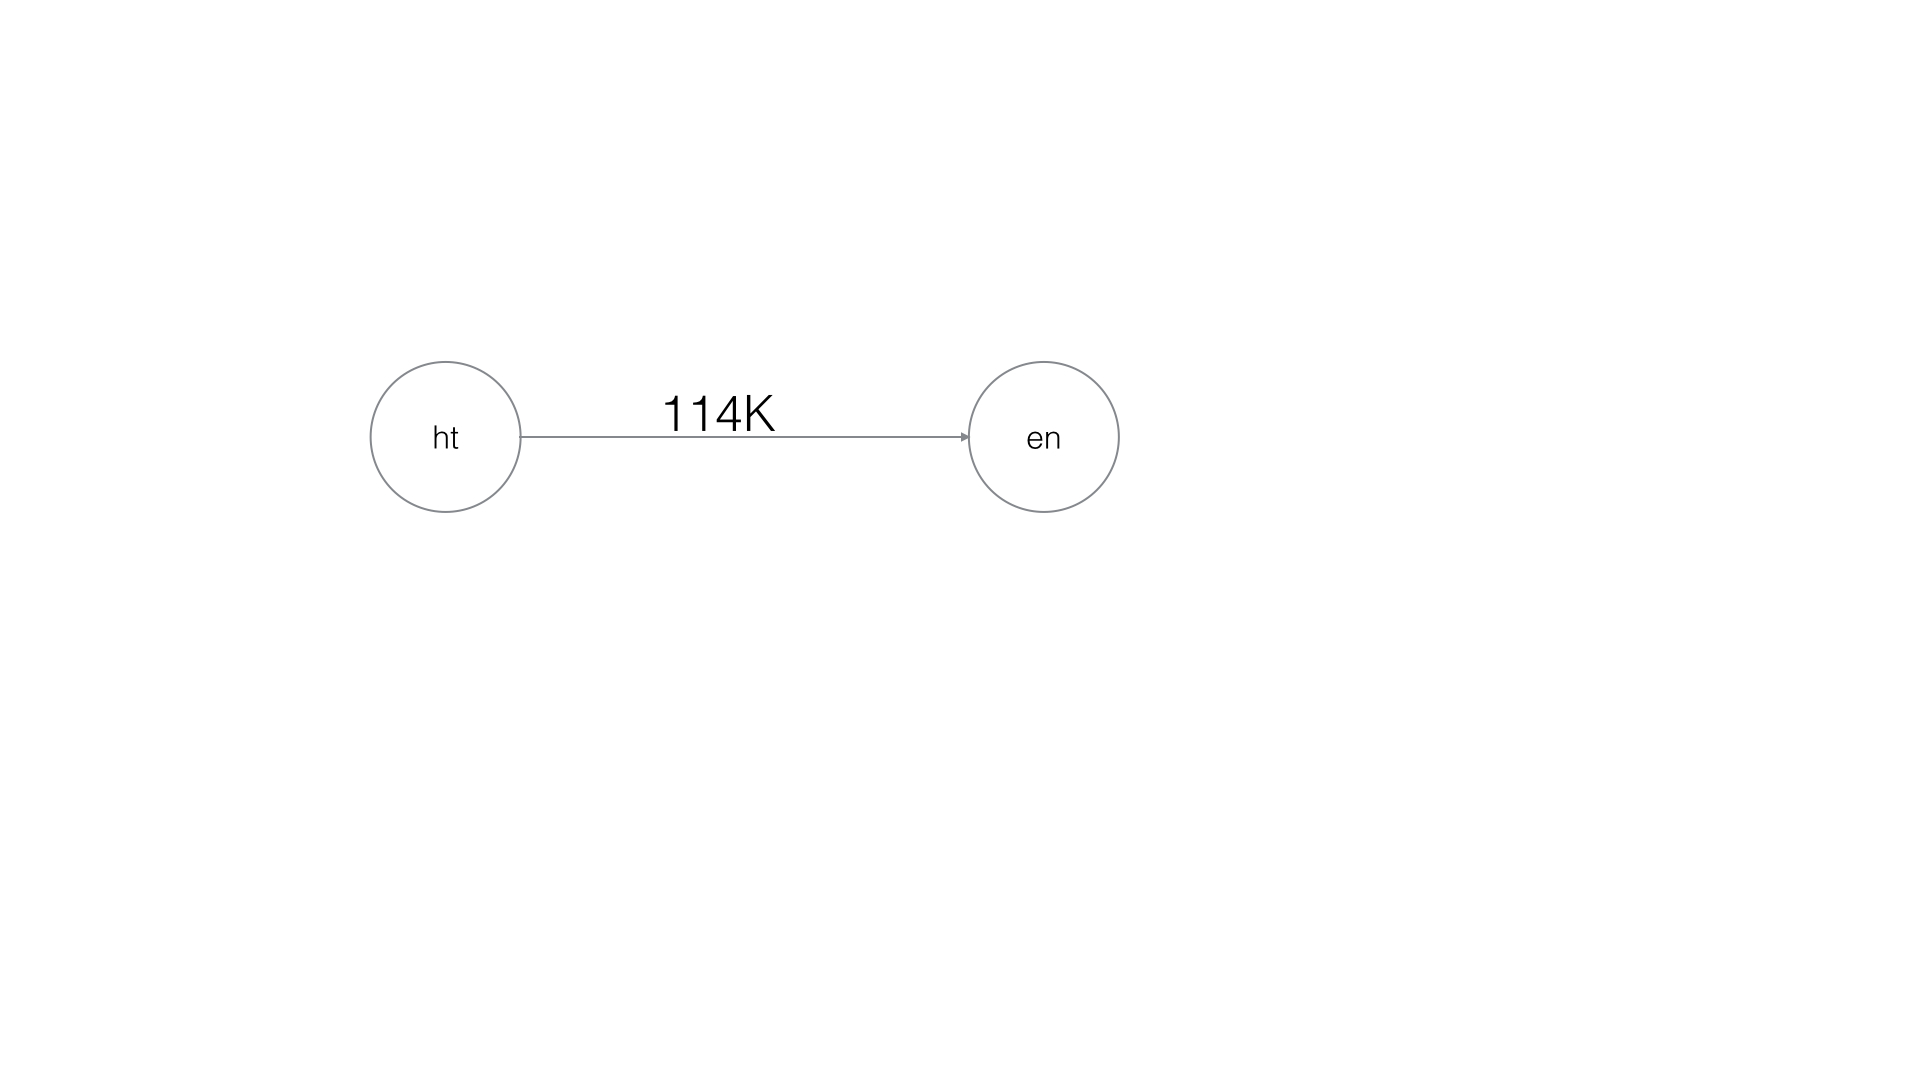
\includegraphics[trim=4cm 4cm 4cm 4cm, clip=true, totalheight=0.5\textheight]{files/Figures/baseline.jpg}
	\caption{Haitian Creole - English baseline}
	\label{fig:training}
\end{figure}

To better understand the effect of the in-domain part of the training data, we report baseline results using various parts of the data, alone and together. A direct Haitian-Creole to English system using just the 15\% of the in-domain training data comfortably beats direct systems trained on a lot more data, in terms of the number of lines, but out-of-domain data. Using all the parallel corpora available to us gives us the best BLEU of all. We also report our baseline using a much larger language model, called \emph{bigLM}. This language model is an interpolation of the English side of the WMT corpus with the english side of Europarl. In all the future experiments, we will use the full-bigLM as our baseline for comparison. 

\begin{figure}[ht]
	\small
	\centering
	\begin{tabular}{lllll} \toprule
System & d(cl) & d(r) & t(cl) & t(r) \\
\toprule
just-ood & 27.56 & 20.77 & 26.72 & 20.14 \\
just-sms & 32.85 & 29.15 & 32.09 & 27.56 \\
full & 33.52 & 29.76 & \emph{33.1} & 28.19 \\
full-bigLM & 33.6 & 29.83 & 33.07 & 28.91 \\ 
\bottomrule
\small
\centering
\label{table:baselines}
\end{tabular}

	\label{fig:haiti_baselines}
	\caption{Baselines - Haitian-Creole to English}
\end{figure}

\section{Mawukakan}
	Mawukakan is one of the four Mandekan languages, the other three being Bambara, Maninkakan and Wojenekakan. Mandekan languages are the Eastern Manding languages of the Mande group of the Niger-Congo family of languages and are small languages, spoken by only half a million people around the world. The Mandekan languages lack a written tradition and hence, have very little representation on the Internet. In this dissertation, we report our results on Maninkakan and Mawukakan to English systems, and the improvements observed when using French as a pivot language. 
	\begin{figure}[ht]
		\small
		\centering
		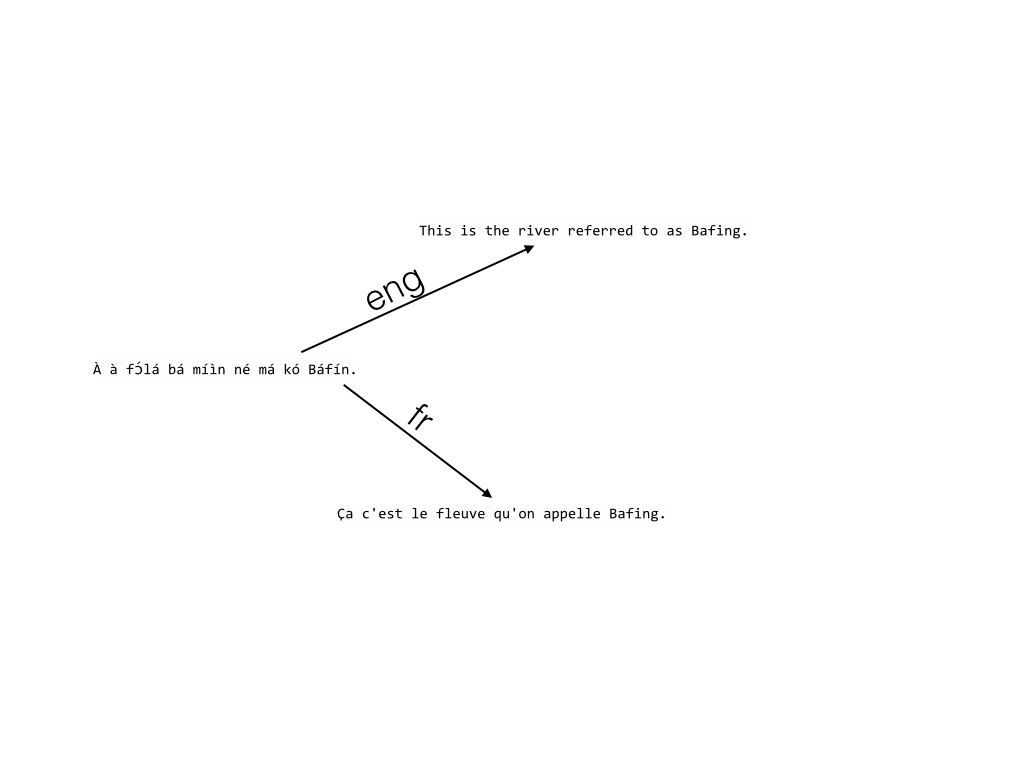
\includegraphics[trim=4cm 1cm 2cm 3cm, clip=true, height=0.6\textheight]{files/Figures/mawu.jpg}
		\caption{Example Mawu - English - French translation}
		\label{fig:mawu_example}
	\end{figure}
	
	\begin{figure}[ht]
		\small
		\centering
		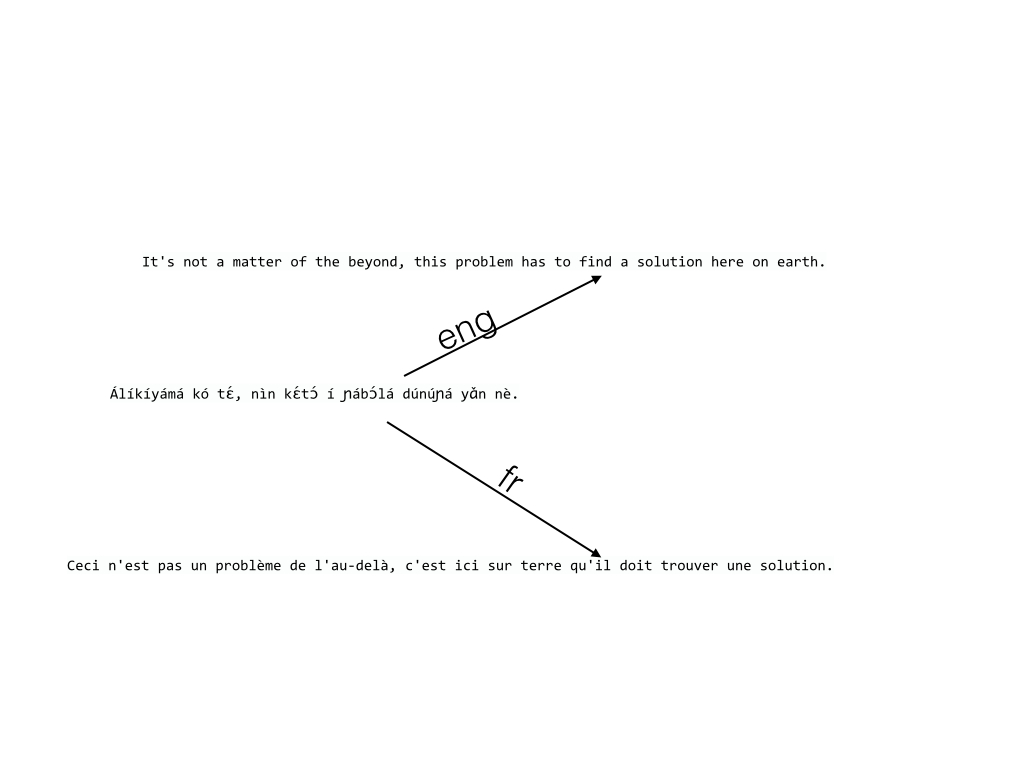
\includegraphics[trim=4cm 2cm 2cm 3cm, clip=true, height=0.6\textheight]{files/Figures/manin.jpg}
		\caption{Example Maninkakan - English - French translation}
		\label{fig:manin_example}
	\end{figure}
	



\section{Remarks}
\label{sec:baseline_remarks}




%!TEX root=/home/ska124/Dropbox/Thesis/thes-full.tex

%%%%%%%%%%%%%%%%%%%%%%%%%%%%%%%%%%%%%%%%%%%%%%%%%
%
%     Chapter 4   
%
%%%%%%%%%%%%%%%%%%%%%%%%%%%%%%%%%%%%%%%%%%%%%%%%

\chapter{Triangulation}
\label{chap:triangulation}

\section{What is Triangulation?}
\label{sec:triangulation}
\alert{Give an example here of each step}



\section{Related Work}
 Consider a source language \emph{s}, pivot language \emph{p} and target language \emph{t}. When using the \emph{cascading} approach, we build two systems, between \emph{s} and \emph{p} and between \emph{p} and \emph{t}. Given a test set in \emph{s}, it is first translated to \emph{p} and those output translations are then translated into the target language \emph{t}, making decoding twice as expensive as well. We do not report our results on using cascading for various reasons. Firstly, translating the output of a source pivot system trained and tuned on little data will lead to propogation of errors. Secondly, we will need three development sets, one for each system. Finding standard development sets for low-resource languages is unlikely. Finally, it has been shown before that cascading does not give the most fluent translations.~\newcite{Utiyama:07} compared pivot-based triangulation with cascading using all of multi-parallel europarl, observing that pivot-based methods outperformed cascading.

 The second approach is the pivot-based approach where a triangulated phrase table is generated between the source and target, by using the common pivot phrases between the source pivot and pivot target tables~\cite{Utiyama:07,Cohn:07}.~\newcite{Utiyama:07} observed that the triangulated table was able to achieve comparable BLEU scores to the direct system for French, German and Spanish. This could be owing to the fact that the data comprised multi-parallel 560K sentences.~\newcite{Cohn:07} observe that multiple pivot languages lead to more fluent translations compared to one pivot language. Multiple pivot language lead to multiple alternative translations, thus, increasing phrase coverage and rewarding the more appropriate translations and reducing out-of-vocabulary words further. They also propose a systematic way of combining the triangulated translation model with the direct model using linear interpolation and log-linear interpolation, although they assume a uniform weight for both the models. To ``simulate'' a low-resource scenario, the top 10K multi-parallel sentences are considered for source pivot, pivot target and source target systems. As we will observe later, real low-resource scenarios are significantly different from how it was simulated in~\cite{Cohn:07}.~\cite{Nakov:12} propose a language-independent approach to improving translation for low-resource languages, but the approach assumes the presence of a resource-rich language that bears similarity to the low-resource language, the similarities helping in creating a large triangulated phrase table. In~\cite{Nakovemnlp:12}, the resource-rich language is adapted to be more like the resource-poor one. Notice that this also assumes both are very similar. Results are reported using both Malay-Indonesian and Bulgarian-Macedonian, the third language being English in both cases.~\cite{Gispert:06} translate Catalan to Spanish via English by using news corpora on both source pivot and pivot target side.~\cite{Huck:12} report on BLEU score improvements by using $10^9$ parallel sentence between German and French.

 
 A common thread that binds the previous work using the approach of Triangulation is the usage of resource-rich languages. The fundamental reason behind the effectiveness of Triangulation is the reduction in the number of OOVs when using the pivot language(s). This can be observed in various forms. If the source and pivot language have a healthy vocabulary overlap, the SMT system between source-pivot is large, thus, improving translations. This factor also helps when the amount of parallel text between source-pivot is relatively low, e.g, Indonesian-English.  All the europarl languages are based on parlimentary proceedings and have minimal noise. Hence, the improvements using triangulation over the direct systems cannot be generalized for systems for low-resource languages. All the papers that use triangulation in machine translation cite either \cite{Utiyama:07} or \cite{Cohn:07}, both published in 2007 (and sometimes cite both of them but use either one model or the other). However, these two papers introduce triangulation for phrase-based SMT in very different ways and their models are different from each other. To our knowledge, before this dissertation, there has been no in-depth study of the different choices in building an SMT system using triangulation. Another limitation of the original work in triangulation~\cite{Utiyama:07,Cohn:07} is the unrealistic use of languages with abundant parallel data to simulate low-resource languages. Subsequent work~\cite{Nakov:12,Nakovemnlp:12,Gispert:06,Huck:12} has also assumed that parallel data in pivot languages can be found in the same domain as the original resource-poor language pair. This kind of domain similarity is not easy to find for realistic low-resource settings.

 ``Simulating'' low-resource scenarios is ineffective in various ways. Firstly, real low-resource languages are noisy, not perfectly sentence aligned, and do not have a lot of data in the target domain. Secondly, triangulation is highly dependent on how good is the source pivot bitext. If the size of source pivot bitext is comparable to the source target, and/or is in the same domain, this increases bias in triangulation by introducting several common phrases, and, this is also not seen in a real low-resource setting.


 Consider a source language, \emph{s}, a target language, \emph{t}, and a pivot language \emph{p}. You have a little parallel data between \emph{s} and \emph{t} and believe that triangulation will increase the quality of translations between \emph{s} and \emph{t}. What steps one would follow to get the desired result ?

\begin{algorithm}
\caption{Triangulate}
\textbf{Input:} phrase table between \emph{s} and \emph{p}, p$_{src-pivot}$, \\
 phrase table between \emph{p} and \emph{t}, p$_{pivot-tgt}$,  \\
 \emph{n} for selecting top-n phrase pairs \\
\textbf{Output:} p$_{trian}$
\begin{algorithmic}
\FORALL{(src, pivot) in top-\emph{n} p$_{src-pivot}$} \IF{pivot phrase in p$_{pivot-tgt}$}

        \FOR{all (pivot, tgt) pairs in p$_{pivot-tgt}$}
        \STATE{find scores for p$_{src-tgt}$}
        \ENDFOR
        \STATE{select top-\emph{n} src-target pair, add to p$_{trian}$}
        \ENDIF
        \ENDFOR


%\ENDFOR
\end{algorithmic}

\end{algorithm}

\begin{equation}
 p_{lex}(t \mid s) = \Sigma p_{lex}(t \mid i) p_{lex}(i \mid s)
\end{equation}

\begin{equation}
	p_{lex}(s \mid t) = \Sigma p_{lex}(s \mid i) p_{lex}(i \mid t)
\end{equation}

\begin{equation}
	p_w(t \mid s) = \Sigma p_w(t \mid i) p_w(i \mid s)
\end{equation}

\begin{equation}
	p_w(s \mid t) = \Sigma p_w(s \mid i) p_w(i \mid t)
\end{equation}

In~\cite{Cohn:07}, 

\begin{eqnarray*}
p(t \mid s)&=&\sum_{i}{p(t, i \mid s)}\\
&=& \sum_{i}{p(t \mid i, s)\,p(i \mid s)}\\
&\approx& \sum_{i}{p(t \mid i)\,p(i \mid s)}
\end{eqnarray*}

\section{Translation Model Combination}
\label{sec:interpolation}

	Combining translation models, trained on corpora from different domains, is an inherently difficult task. We want to make our translations better on the domain of the test set, while also correcting errors in our baseline translation model. In case of low-resource languages, the baseline translation model has been trained on completely out-of-domain corpora or some in-domain and a lot of out-of-domain corpora. This results in translation pairs that are missing altogether or translation pairs with so low probability that decoding misses them altogether. The aim of Interpolation is to add translation pairs that are missing and give more weightage to translations that are more valid in the given domain. 

	Consider the translations from Haitian-Creole to English. We have a baseline model trained on a little in-domain parallel data (\~17K sentences). We aim to make our translations better on the same domain using a lot of out-of-domain data, which in our case is parlimentary proceedings. Its important that we do not make the baseline model translations end up at the bottom of the stack because they are in-domain. At the same time, we do not want to miss out on the valid translations introduced by the larger, clean parliamentary proceedings based translation model. 

	\subsection{Example}
		Consider a phrase pair, (jan nou, that you). Each phrase pair has a set of scores associated with it in the phrase table. They are the forward and backward lexical probabilities, and the forward and backward phrase probabilities. 

		From the direct phrase table, we have the following scores for the phrase pair mentioned above. The last score, 2.718, is a constant which is the phrase penalty. 
	\begin{verbatim}
		jan nou  ||| that you ||| 0.000786782 2.11603e-05 0.125 0.00906772 2.718 
	\end{verbatim}

		The triangulated table also happens to have the same phrase pair with different scores. These scores have been obtained by using the equations shown above.
	\begin{verbatim}
		jan nou ||| that you ||| 0.00318015 7.75194e-05 0.0715829 0.00214831 2.718
	\end{verbatim}

		We know that our direct system has been trained on in-domain data, hence, it should get more weightage intuitively. A heuristic approach to this problem would choose a pair of values and see which one does best. For instance, if you choose 0.85 for the direct table and 0.15 for the triangulated table, the end result for the phrase pair would look like the following : 

	\begin{verbatim}
		jan nou ||| that you ||| 0.0011457872 2.961416503e-05 0.116987435 0.00802980849 2.718	
	\end{verbatim}

		There are several flaws with the approach outlined above. Firstly, an intuitive idea about the importance of the in-domain or out-of-domain phrase table is not enough. The direct Haitian-creole to English phrase table has been trained on only 110K parallel sentences and cannot always be right. Hence, starting with 0.9 for the direct table and 0.1 for the triangulated table is an extreme step. So is 0.5 and 0.5 because we want translations with more influence from the cleaner, larger Europarl data. Moreover, as we will discuss in the other chapters, we report results on several combinations of triangulation, based on changes in phrase scores, lexical scores and adding connectivity features. With every improvement, the importance of the triangulated table might increase or decrease. The heuristic approach will not be able to take that into account. 

		We use CONDOR to perform an efficient grid search over the pairs of co-efficients based on the BLEU score of the interpolated system on the heldout set. Our intepolation method would have the following steps : 
 
		\begin{itemize}
			\item Start with a number, say, 0.85 and 0.15
			\item Interpolate baseline and triangulated. Run MERT with the interpolated table
			\item Get the BLEU of this set of weights on heldout set
			\item Based on the BLEU score, Condor generates a new pair of co-efficients
		\end{itemize}



\section{Europarl}
Europarl refers to the parallel corpora generated by translating the proceedings of European parliament into several languages. Version 7 of Europarl now has 20 languages, from French to Estonian and Finnish. Release of the Europarl corpus led to a surge in research into more and more data-driven methods to enable Statistical Machine Translation. The results were easily reproducible and the data is very clean and sentence-aligned. 

Moreover, Europarl is multi-parallel. What does multi-parallel imply? Consider english as the common target language. A multi-parallel corpora between 20 European languages and English comprises sentences in 20 european languages which translate to the same english sentence. 

\begin{figure}[ht]
	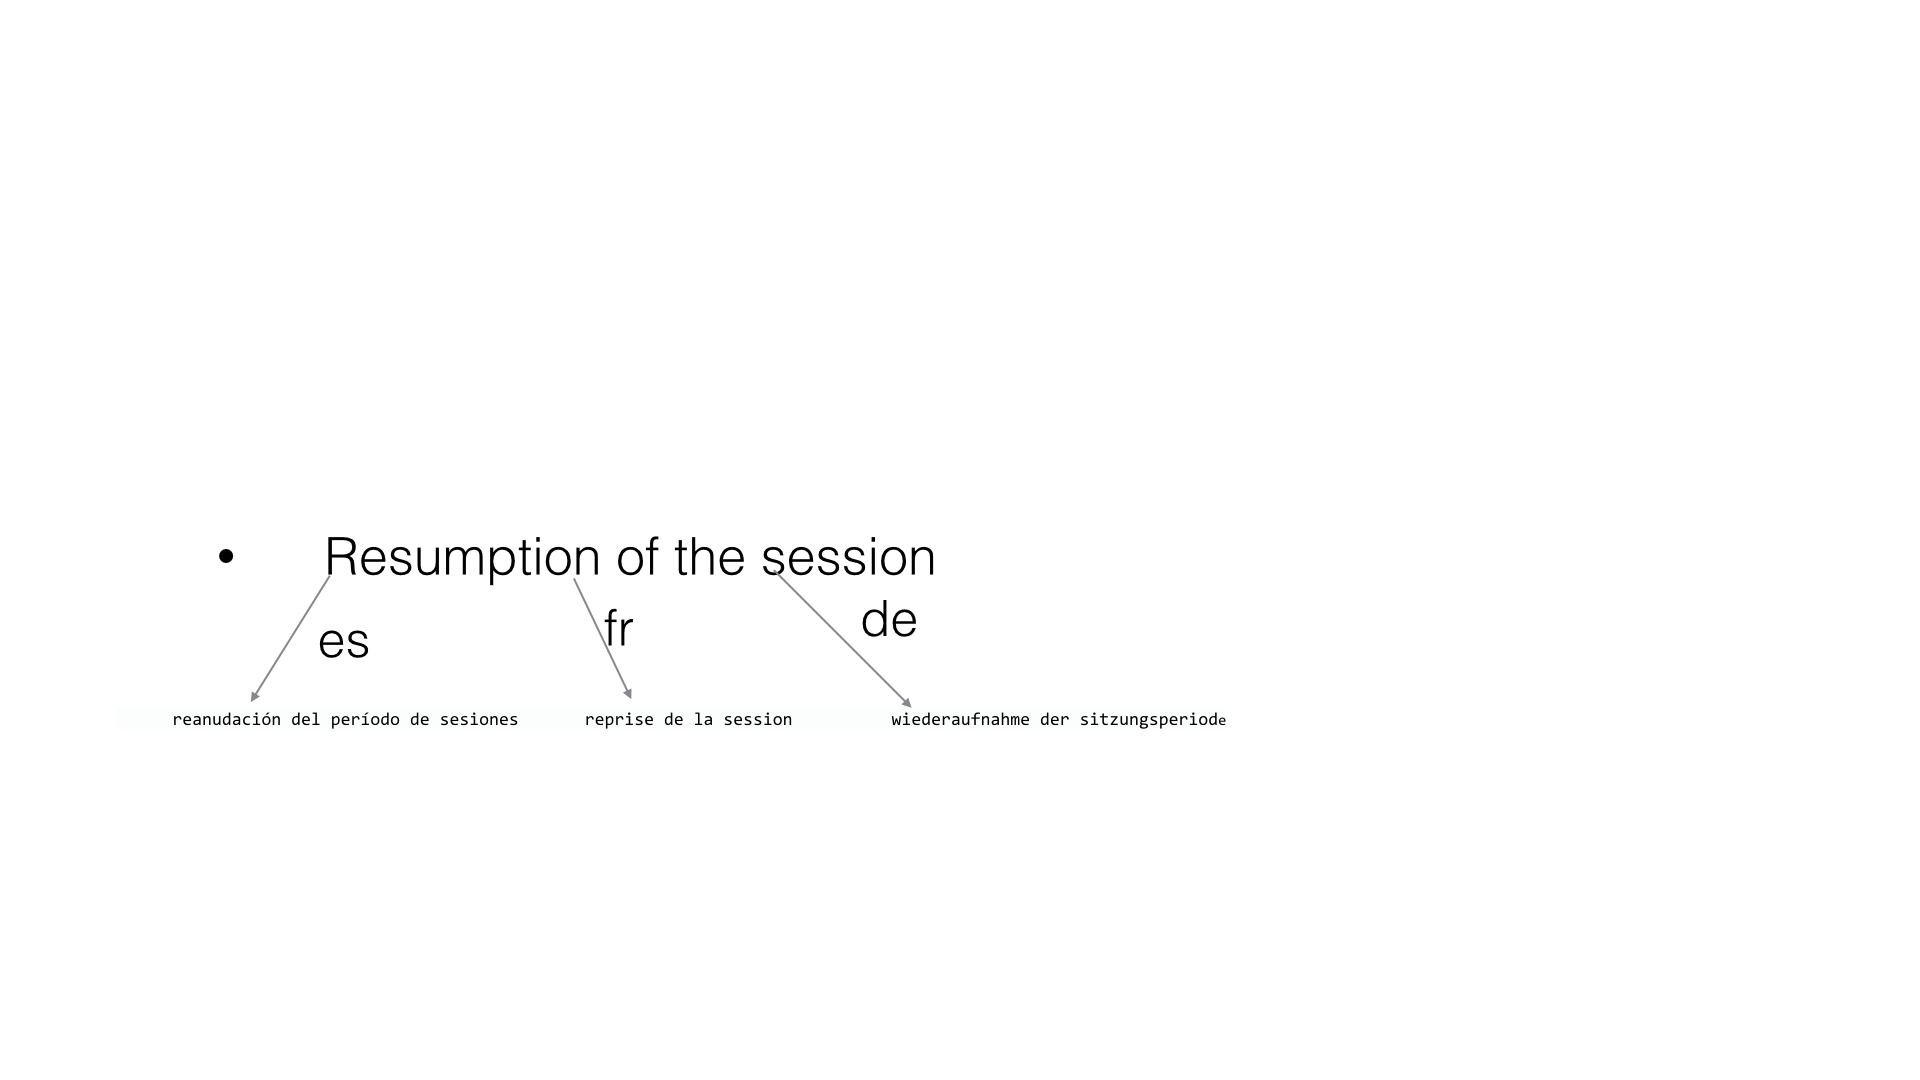
\includegraphics[trim=4cm 4cm 4cm 4cm, height=0.5\textheight, clip=true]{files/Figures/eparl_multiparallel.jpg}
	\caption{Spanish = es, French = fr, German = de}
	\label{fig:eparl_multi}
	\small
	\centering
\end{figure}



\section{Low-resource simulation}

\cite{Cohn:07} simulated ``low-resource'' settings by using the top 10K sentences for the source pivot, pivot target and source target systems.  

\begin{figure}[ht]
	\small
	\centering
	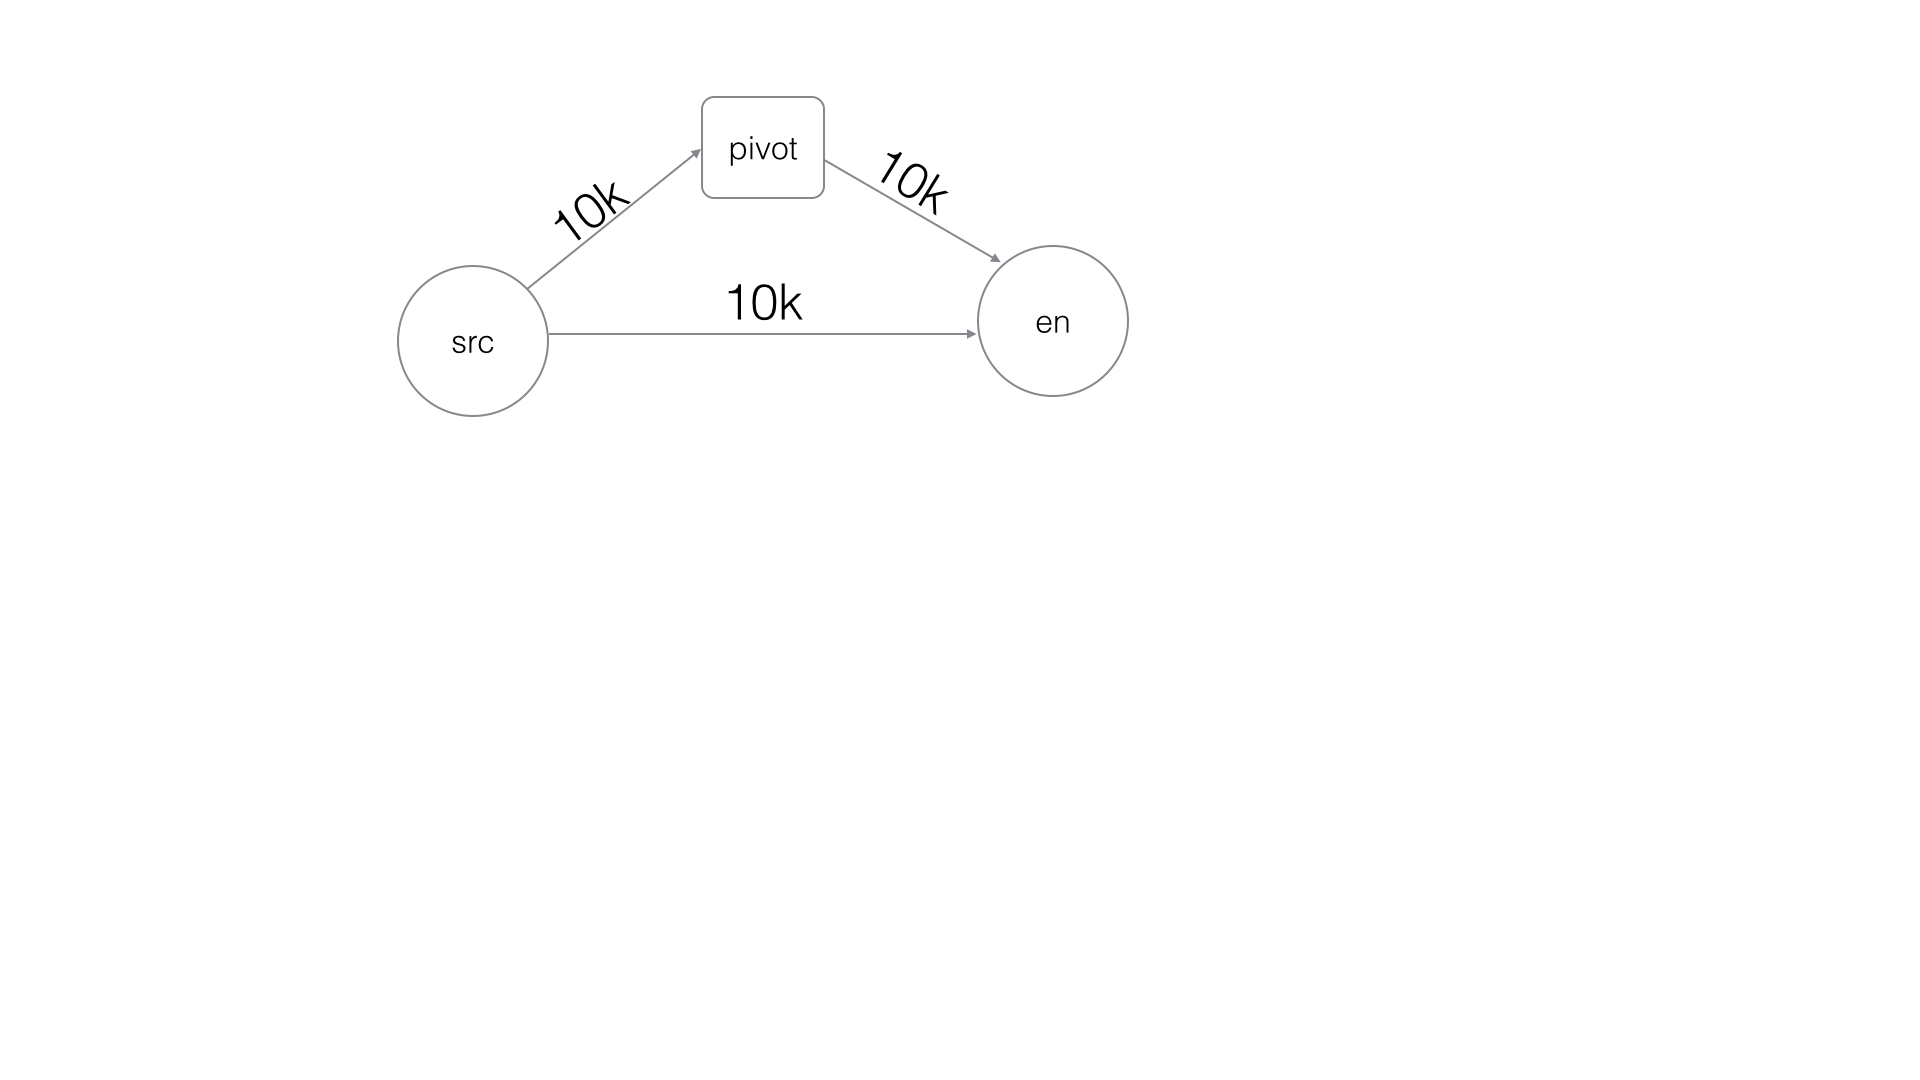
\includegraphics[trim=2cm 4cm 4cm 4cm, height=0.6\textheight]{files/Figures/Cohn.jpg} 
	\caption{Low-resource simulation in Cohn \& Lapata, '07}
	\label{fig:Cohn_lowresource}
\end{figure}

\begin{figure}
	\small
	\centering
	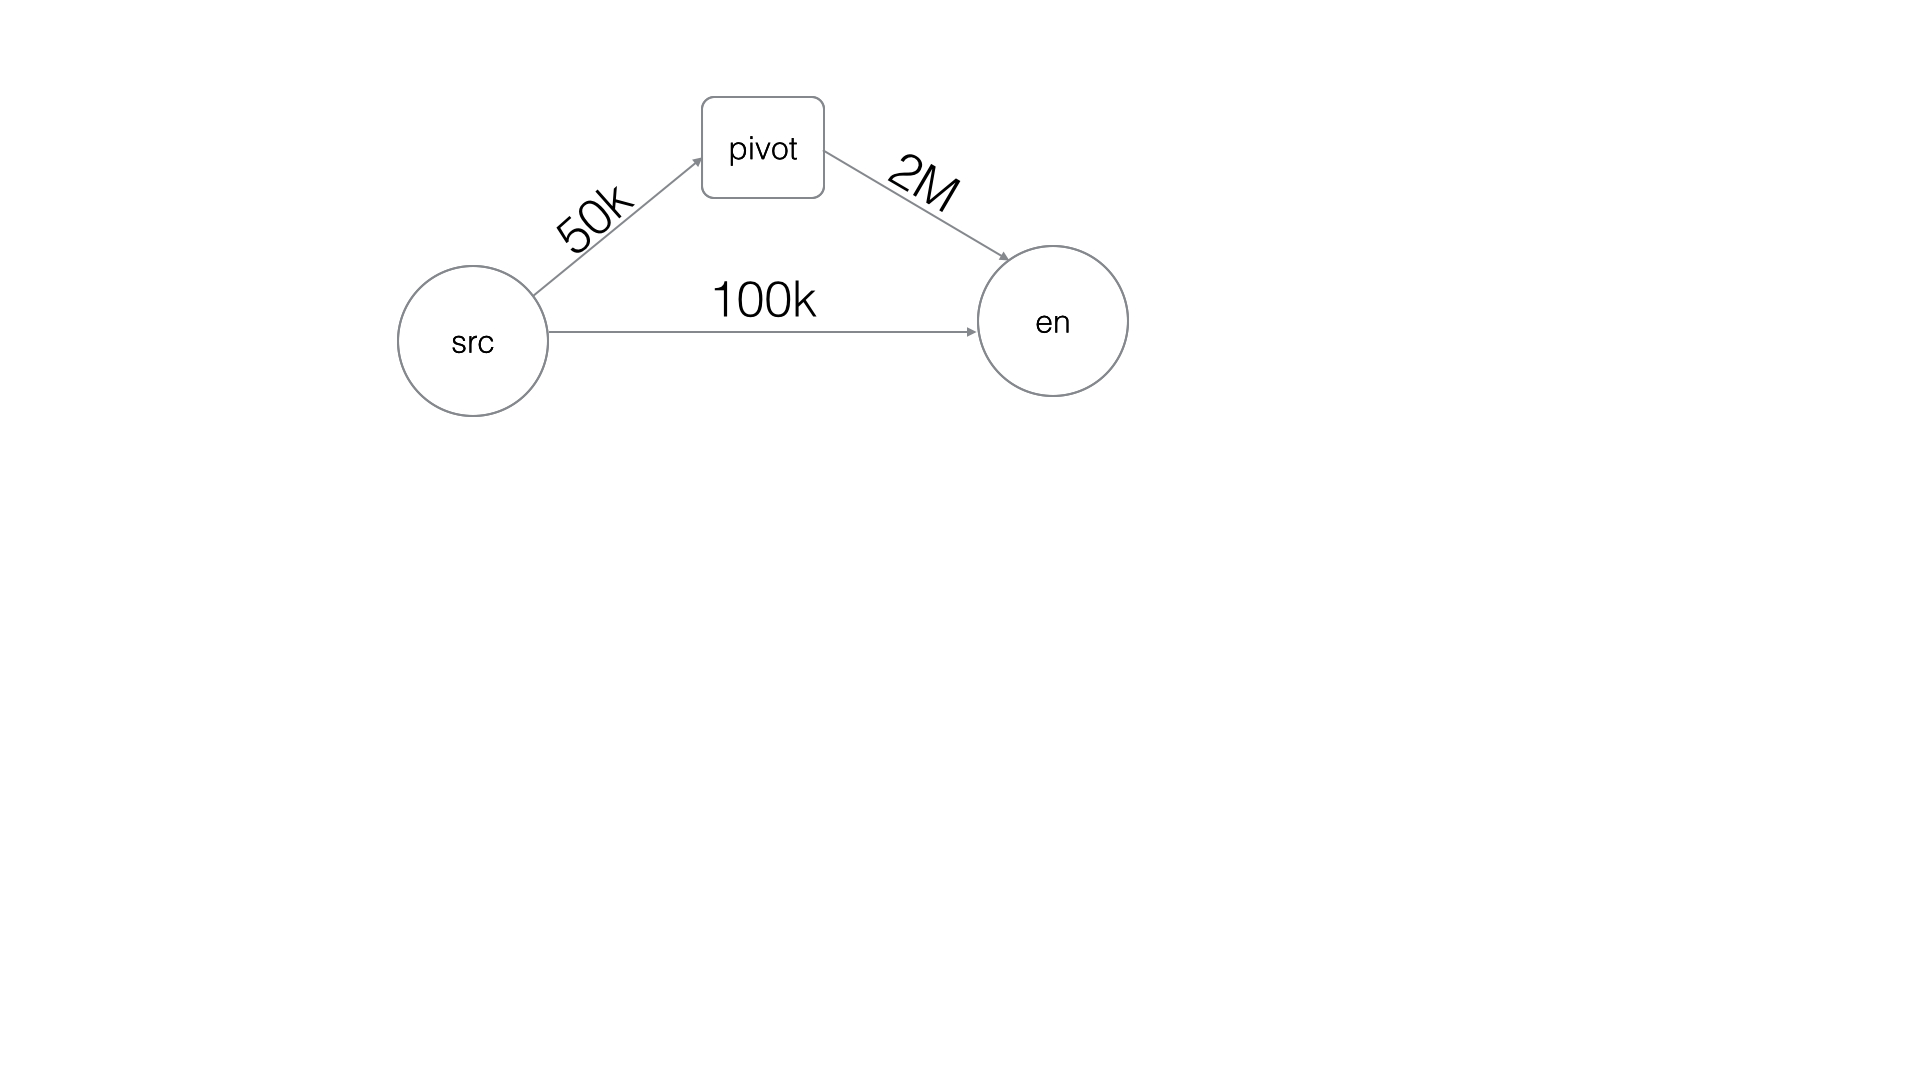
\includegraphics[trim=2cm 4cm 4cm 4cm, height=0.5\textheight]{files/Figures/Our.jpg} 
	\caption{Our low-resource simulation setting}
	\label{fig:our_setting}
\end{figure}



\section{Experiments}
\begin{figure}[ht]
	\small
	\centering

	\begin{tabular}{lr}

\toprule
System & BLEU \\
\toprule
es-en & 23.32 \\
fr-en & 19.53 \\
de-en & 15.60 \\
\bottomrule
\centering
\small
\label{table:eparl100}
\end{tabular}
	\label{table:eparlbaselines}
	\caption{Europarl Baselines - 100K}
\end{figure}

 \begin{figure}[ht]
 	\small
 	\centering
	\begin{tabular}{lrrrrrr}
\toprule

src-tgt & pivot & top20 & top40 & top60 & top80 & top100 \\
\toprule

de-en & fr & 13.32 & 13.33 & 13.35 & 13.42 & 13.03 \\
de-en & es & 13.37 & 13.17 & 13.49 & 13.34 & 13.36 \\
fr-en & de & 16.21 & 15.82 & 15.89 & 16.08 & - \\
fr-en & es & 17.77 & 18.15 & 17.99 & 18.01 & 18.27 \\
es-en & fr & 21.35 & 21.18 & 20.83 & 21.01 & 21.45\\
es-en & de & 18.36 & 19.19 & 19.35 & 19.23 & 18.97 \\
\bottomrule
\centering 
\small
\label{table:eparltopn}
\end{tabular}
 
	\label{table:eparltopn}
	\caption{BLEU scores when just using the triangulated table}
 \end{figure}


\section{Translation Model Combination}

\begin{figure}[ht]
	\small
	\centering
	\begin{tabular}{llrrrrrr}
\toprule
src-tgt & pivot & baseline & top20 & strength & M1 & joint & all \\
\toprule
de-en & fr & 15.60 & 15.45 & - & 15.24 & - & -  \\
de-en & es & 15.60 & 15.55 & - & 15.49 & - & - \\
fr-en & de & 19.53 & 19.85 & - & 19.92 & - & - \\
fr-en & es & 19.53 & 19.86 & - & 20.03 & - & - \\
es-en & fr & 23.32 & 23.66 & - & 23.85 & - & - \\
es-en & de & 23.32 & 23.68 & - & 23.84 & - & - \\
\bottomrule
\centering
\small
\label{table:eparlintertopn}
\end{tabular}
	\label{table:eparltopninter}
	\caption{BLEU scores with top-20 interpolation}
\end{figure}




%\section{Using Bible}

%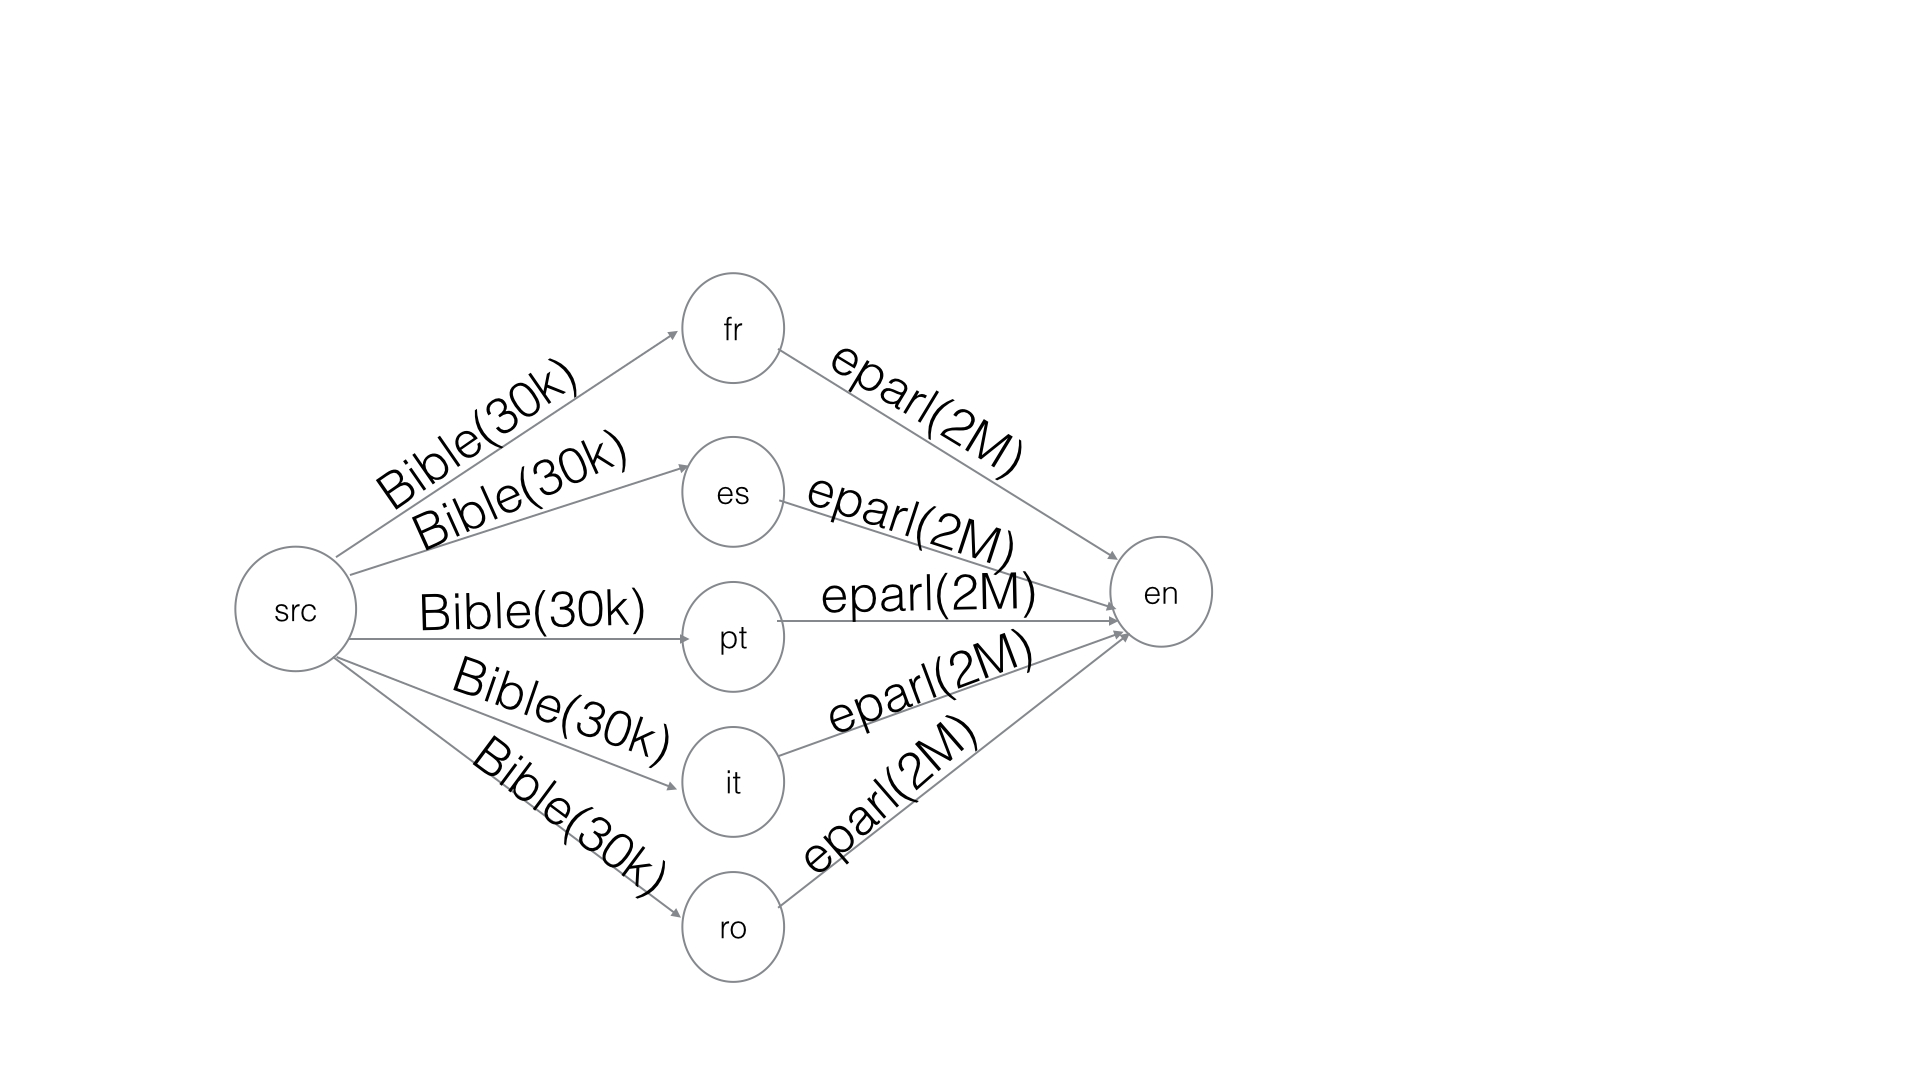
\includegraphics[scale=0.4]{files/Figures/pivot.jpg}






%!TEX root=/home/ska124/Dropbox/Thesis/thes-full.tex

%%%%%%%%%%%%%%%%%%%%%%%%%%%%%%%%%%%%%%%%%%%%%%%%%
%
%     Chapter 5
%
%%%%%%%%%%%%%%%%%%%%%%%%%%%%%%%%%%%%%%%%%%%%%%%%

\chapter{Design Choices}
\label{chap:design_choices}


\begin{figure}[ht]
	\small
	\centering
	


% Set the overall layout of the tree
\tikzstyle{level 1}=[level distance=3.5cm, sibling distance=3.5cm]
\tikzstyle{level 2}=[level distance=3.5cm, sibling distance=2cm]

% Define styles for bags and leafs
\tikzstyle{bag} = [text width=4em, text centered]
\tikzstyle{end} = [circle, minimum width=3pt,fill, inner sep=0pt]

% The sloped option gives rotated edge labels. Personally
% I find sloped labels a bit difficult to read. Remove the sloped options
% to get horizontal labels. 
\begin{tikzpicture}[grow=right, sloped][scale=0.4]
\node[bag] {33.6}
	child {
		node[bag] {34.11}
		child {
			node[end, label = left:
			{}] {}
			edge from parent 
			node[above] {strength}
		}
		child {
			node[end, label = left:
			{}] {}
			edge from parent
			node[below] {M1-sub}
		}
		edge from parent
		node[above] {romance * 5}
	}
	child {
		node[bag] {33.84}
	child {
		node[bag] {33.92}
			child {
				node[end, label = right:
				 {33.76}] {}
				edge from parent 
				node[above] {+loglin * 2}
				}
			child {
				node[end, label = right:
				{33.85}] {}
				edge from parent
				node[above] {-lex*2, +m1*2}
			}
		edge from parent
		node[above] {+strength*2}
	}
	child {
		node[end, label = right:
		{\textbf{34.00}}] {}
		edge from parent 
		node[above] {+m1*2, -lex*2}
	}
    child {
        node[bag] {33.78}        
            child {
                node[end, label=right:
                    {33.65}] {}
                edge from parent
                node[above] {joint + dec*2}
            }
            edge from parent
            node[above] {+loglin*2}
    }
    edge from parent
    node[above] {+top20}
    };
   
        
\end{tikzpicture}


	\label{fig:ht_tikz}
	\caption{Diagram of Haiti}
\end{figure}


\begin{figure}[ht]
	\small
	\centering
	


% Set the overall layout of the tree
\tikzstyle{level 1}=[level distance=3.5cm, sibling distance=3.5cm]
\tikzstyle{level 2}=[level distance=3.5cm, sibling distance=2cm]

% Define styles for bags and leafs
\tikzstyle{bag} = [text width=4em, text centered]
\tikzstyle{end} = [circle, minimum width=3pt,fill, inner sep=0pt]

% The sloped option gives rotated edge labels. Personally
% I find sloped labels a bit difficult to read. Remove the sloped options
% to get horizontal labels. 
\begin{tikzpicture}[grow=right, sloped][scale=0.4]
\node[bag] {18.81}
	child {
		node[bag] {-}
		child {
			node[end, label = left:
			{-}] {}
			edge from parent 
			node[above] {strength}
		}
		child {
			node[end, label = left:
			{-}] {}
			edge from parent
			node[below] {M1-sub}
		}
		edge from parent
		node[above] {romance * 5}
	}
	child {
		node[bag] {-}
	child {
		node[bag] {19.03}
			child {
				node[end, label = right:
				 {-}] {}
				edge from parent 
				node[above] {+loglin * 2}
				}
			child {
				node[end, label = right:
				{-}] {}
				edge from parent
				node[above] {-lex*2, +m1*2}
			}
		edge from parent
		node[above] {+strength*2}
	}
	child {
		node[end, label = right:
		{\textbf{19.20}}] {}
		edge from parent 
		node[above] {+m1*2, -lex*2}
	}
    child {
        node[bag] {-}        
            child {
                node[end, label=right:
                    {-}] {}
                edge from parent
                node[above] {joint + dec*2}
            }
            edge from parent
            node[above] {+loglin*2}
    }
    edge from parent
    node[above] {+top20}
    };
   
        
\end{tikzpicture}


	\label{fig:mlg_tikz}
	\caption{Malagasy Diagram}
\end{figure}


\begin{figure}[ht]
	\small
	\centering
	


% Set the overall layout of the tree
\tikzstyle{level 1}=[level distance=3.5cm, sibling distance=3.5cm]
\tikzstyle{level 2}=[level distance=3.5cm, sibling distance=2cm]

% Define styles for bags and leafs
\tikzstyle{bag} = [text width=4em, text centered]
\tikzstyle{end} = [circle, minimum width=3pt,fill, inner sep=0pt]

% The sloped option gives rotated edge labels. Personally
% I find sloped labels a bit difficult to read. Remove the sloped options
% to get horizontal labels. 
\begin{tikzpicture}[grow=right, sloped][scale=0.2]
\node[bag] {5.99(5.75)}
	child {
		node[end, label = right:
		{8.56}] {}
		edge from parent
		node[above] {strength}
	}
	child {
		node[end, label = right:
		{-}] {}
		edge from parent
		node[above] {strength-100}
	}
	child {
		node[end, label = right:
		{8.46}] {}
		edge from parent
		node[above] {top-100}
	}
	child {
		node[end, label = right:
		{-}] {}
		edge from parent
		node[above] {M1-100}
	}
	child {
		node[end, label = right:
		{8.57}] {}
		edge from parent
		node[above] {top20}
	}
	child {
		node[end, label = right:
		{8.55}] {}
		edge from parent
		node[above] {M1}
	}
	child {
		node[end, label = right:
		{-}] {}
		edge from parent 
		node[above] {Joint}
	};
    
        
\end{tikzpicture}


	\label{fig:mawu_tikz}
	\caption{Mawu Diagram}
\end{figure}

\begin{figure}[ht]
	\small
	\centering
	


% Set the overall layout of the tree
\tikzstyle{level 1}=[level distance=3.5cm, sibling distance=3.5cm]
\tikzstyle{level 2}=[level distance=3.5cm, sibling distance=2cm]

% Define styles for bags and leafs
\tikzstyle{bag} = [text width=4em, text centered]
\tikzstyle{end} = [circle, minimum width=3pt,fill, inner sep=0pt]

% The sloped option gives rotated edge labels. Personally
% I find sloped labels a bit difficult to read. Remove the sloped options
% to get horizontal labels. 
\begin{tikzpicture}[grow=right, sloped][scale=0.4]
\node[bag] {9.96}
	child {
		node[end, label = right:
		{10.76}] {}
		edge from parent
		node[above] {strength}
	}
	child {
		node[end, label = right:
		{10.85}] {}
		edge from parent
		node[above] {strength-100}
	}
	child {
		node[end, label = right:
		{10.76}] {}
		edge from parent
		node[above] {top20}
	}
	child {
		node[end, label = right:
		{11.03}] {}
		edge from parent
		node[above] {top100}
	}
	child {
		node[end, label = right:
		{-}] {}
		edge from parent
		node[above] {m1-100}
	}
	child {
		node[end, label = right:
		{10.57}] {}
		edge from parent
		node[above] {M1}
	}
	child {
		node[end, label = right:
		{-}] {}
		edge from parent 
		node[above] {Joint}
	};
    
        
\end{tikzpicture}


	\label{fig:manin_tikz}
	\caption{Manin Diagram}
\end{figure}

\begin{comment}
\begin{figure}[ht]
	\small
	\centering
	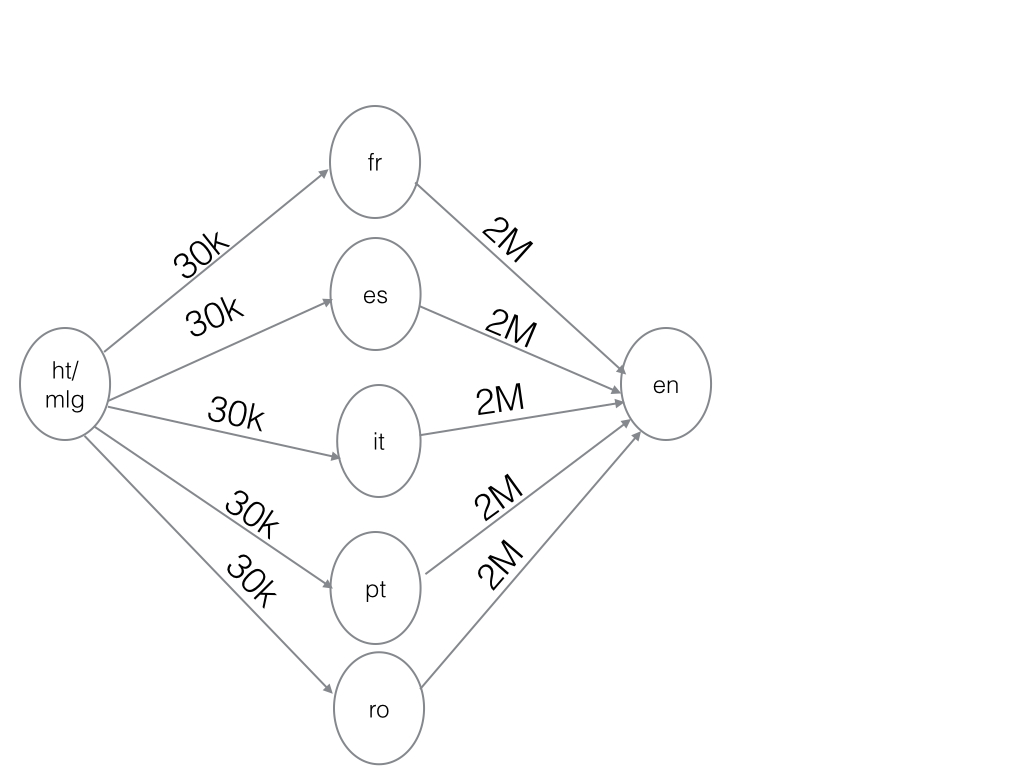
\includegraphics[height=0.5\textheight]{files/Figures/data_multi_pivot.jpg}
	\label{fig:multi_pivots}
	\caption{ht=Haitian-Creole, mlg=Malagasy, en=English, \{fr, it, pt, ro, es\} are the pivot languages}
\end{figure}
\section{Top-n filtering}
\label{sec:topn}

	\subsection{Haitian-Creole}
	\begin{table*}\centering
\small
\begin{tabular}{cllllllclllllll} \toprule
& \multicolumn{6}{c}{$d(cl)$} & \phantom{a} & \multicolumn{6}{c}{$d(r)$} & \phantom{a} \\
\cmidrule{2-7} \cmidrule{9-14} 
& $fr$ & $es$ & $it$ & $pt$ & $ro$ & $\emph{All}$ && $fr$ & $es$ & $it$ & $pt$ & $ro$ & $\emph{All}$  \\
\toprule
$n=20$\\
$$ & 19.84 & 17.21 & 7.29 & - & 9.62 & - && 16.11 & 13.72 & 6.99 & - & 7.98 & -  \\ \toprule
$n=40$ \\
$$ & 19.81 & 17.82 & 7.74 & - & 3.97 & - && 15.92 & 13.80 & 7.36 & - & 3.97 & -  \\ \toprule 
$n=60$ \\
$$ & 20.06 & 17.83 & 6.90 & - & 8.37 & - && 15.96 & 13.76 & 6.98 & - & 7.72 & -  \\ \toprule 
$n=80$ \\
$$ & 19.45 & 16.80 & 4.94 & - & 8.09 & - && 15.36 & 13.46 & 4.91 & - & 7.50 & -  \\
\toprule
$n=100$ \\
$$ & 19.68 & 17.37 & 7.11 & - & - & - && 15.37 & 13.40 & - & 7.01 & - & -  \\
\bottomrule
\end{tabular}
\caption{fr, es, pt, it, ro are the pivot languages, \emph{all} = fr + es + it + pt + ro, d= devtest, cl= clean, r= raw}
\end{table*} 



	\begin{figure}[p]
		\centering
		
\includegraphics[width=\columnwidth]{files/Figures/multi_ht.png}
		\caption{Multiplication Factors: Haitian-Creole}
		\label{fig:multi_ht}
	\end{figure}
	\subsection{Malagasy}


\section{Lexical scores}
\label{sec:lexical_scores}
	\subsection{Haitian-Creole}
	\subsection{Malagasy}

\section{Strength features}
\label{sec:strength_features}
	\subsection{Haitian-Creole}
	\begin{table*}\centering
\small
\begin{tabular}{cllllllclllllll} \toprule
& \multicolumn{6}{c}{$d(cl)$} & \phantom{a} & \multicolumn{6}{c}{$d(r)$} & \phantom{a} \\
\cmidrule{2-7} \cmidrule{9-14} 
& $fr$ & 
$es$ & 
$it$ & 
$pt$ & 
$ro$ & 
$\emph{All}$ && 
$fr$ & 
$es$ & 
$it$ & 
$pt$ & 
$ro$ & 
$\emph{All}$  \\
\toprule
$n=20$\\
$$ & 
19.63 & 
17.50 & 
7.29 & 
7.87 & 
9.90 & 
- && 
15.81 & 
13.70 & 
6.99 & 
7.38 & 
8.23 & 
-  \\ \toprule
$n=40$ \\
$$ & 
20.09 & 
- & 
- & 
2.72 & 
9.60 & 
- && 
16.24 &  
- & 
- & 
2.10 & 
8.12 &
 -  \\ \toprule 
$n=60$ \\
$$ & 
19.57 & 
17.96 & 
7.02 & 
- & 
9.05 & 
- && 
16.07 & 
14.17 & 
7.29 & 
- & 
7.89 & 
-  \\ \toprule 
$n=80$ \\
$$ & 
19.66 & 
15.09 & 
8.15 & 
- & 
- & 
- && 
15.96 & 
12.89 & 
7.89 & 
- & 
- & 
-  \\
\toprule
$n=100$ \\
$$ & 
18.95 & 
13.72 & 
7.40 & 
- & 
9.93 & 
- && 
16.00 & 
11.14 & 
6.91 & 
- & 
8.80 & 
-  \\
\bottomrule
\end{tabular}
\caption{fr, es, pt, it, ro are the pivot languages, \emph{all} = fr + es + it + pt + ro, d= devtest, cl= clean, r= raw}
\end{table*} 


	\subsection{Malagasy}

\section{Phrase scores}
\label{sec:phrase_scores}
	\subsection{Haitian-Creole}
	\subsection{Malagasy}

\section{All-features}
\label{sec:hail_mary}

\section{Multiple pivots}
\label{sec:multiple}

\section{Results}
\label{sec:improved_results}
\end{comment}



%%!TEX root=/home/ska124/Dropbox/Thesis/thes-full.tex

%%%%%%%%%%%%%%%%%%%%%%%%%%%%%%%%%%%%%%%%%%%%%%%%%
%
%     Chapter 6
%
%%%%%%%%%%%%%%%%%%%%%%%%%%%%%%%%%%%%%%%%%%%%%%%%

\chapter{Detour: Europarl}
\label{chap:europarl}

\section{What is Europarl?}
Europarl refers to the parallel corpora generated by translating the proceedings of European parliament into several languages. Version 7 of Europarl now has 20 languages, from French to Estonian and Finnish. Release of the Europarl corpus led to a surge in research into more and more data-driven methods to enable Statistical Machine Translation. The results were easily reproducible and the data is very clean and sentence-aligned. 

Moreover, Europarl is multi-parallel. What does multi-parallel imply? Consider english as the common target language. A multi-parallel corpora between 20 European languages and English comprises sentences in 20 european languages which translate to the same english sentence. 

\begin{figure}
	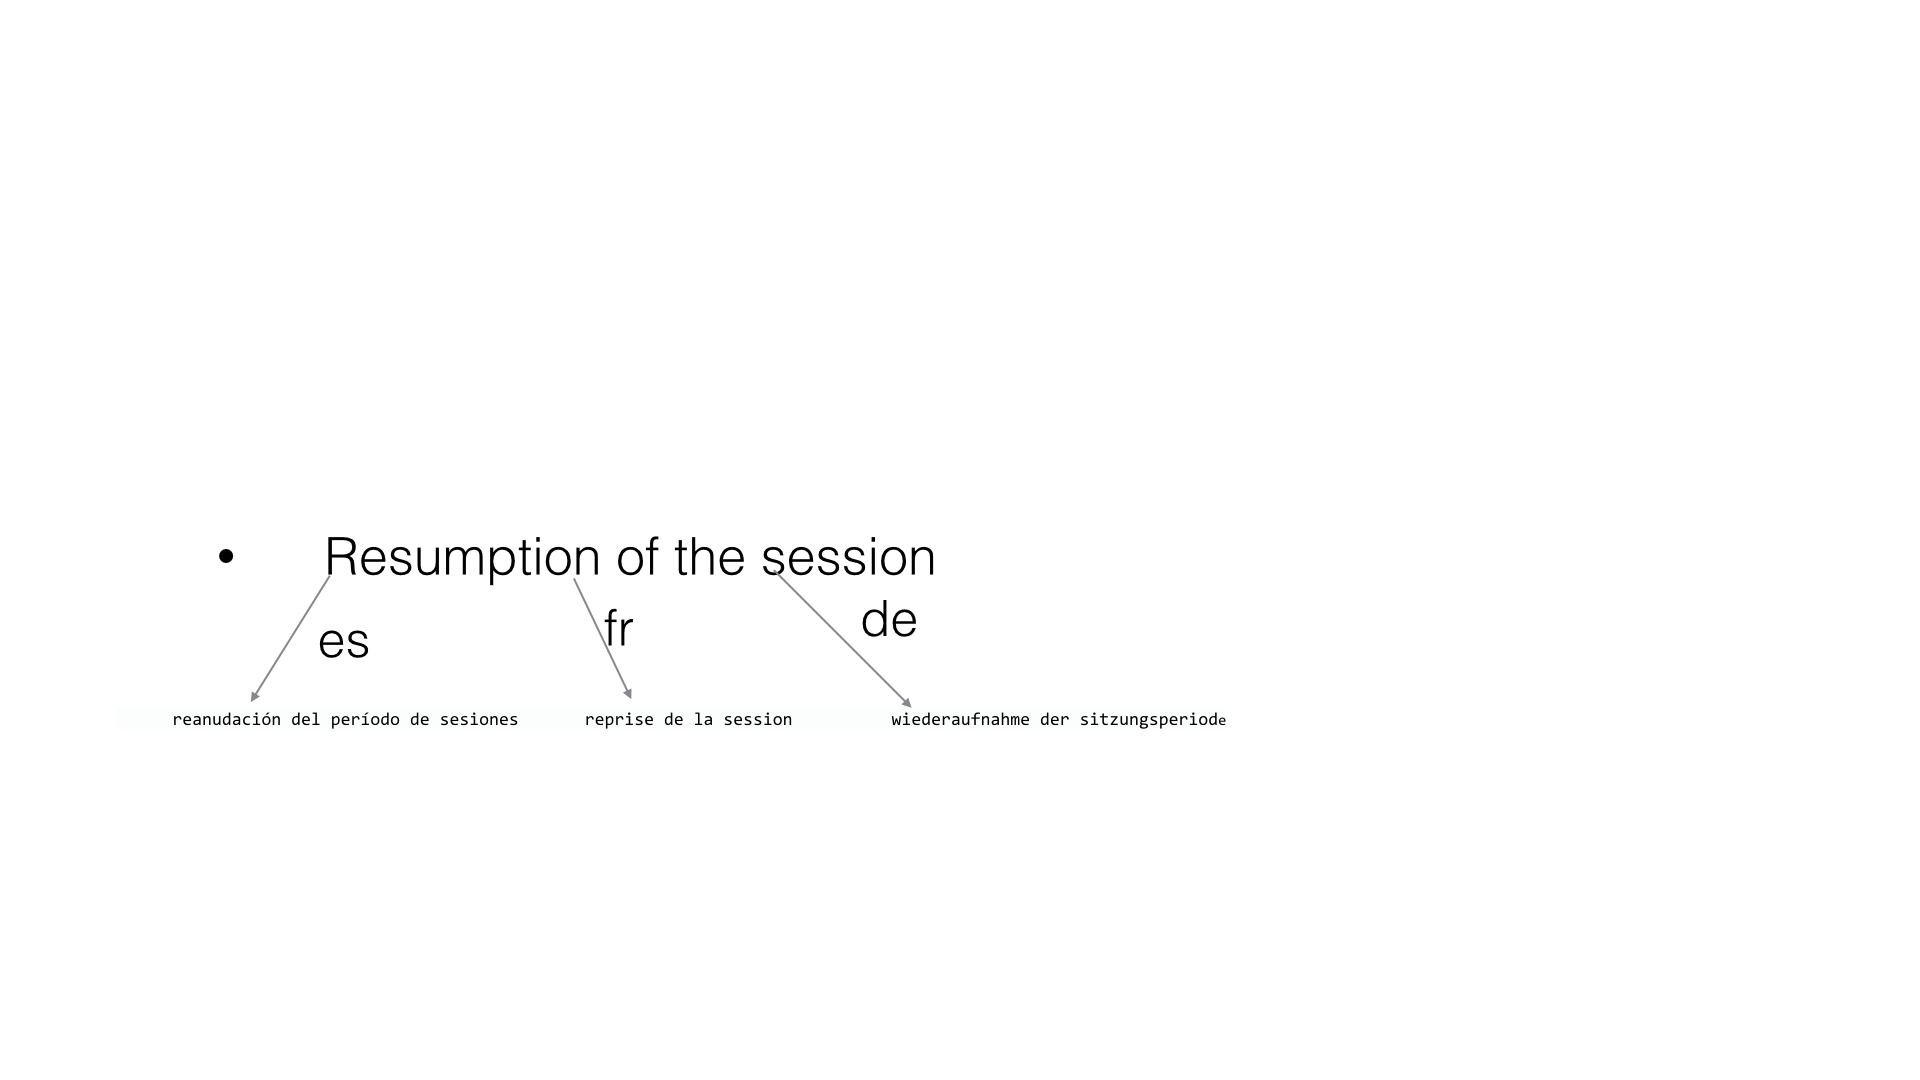
\includegraphics[scale=0.4]{files/Figures/eparl_multiparallel.jpg}
	\caption{Spanish = es, French = fr, German = de}
	\label{fig:eparl_multi}
\end{figure}


\section{Triangulation for Europarl languages}



\section{How best to simulate low-resource?}

~\cite{Cohn:07} simulated ``low-resource'' settings by using the top 10K sentences for the source pivot, pivot target and source target systems.  

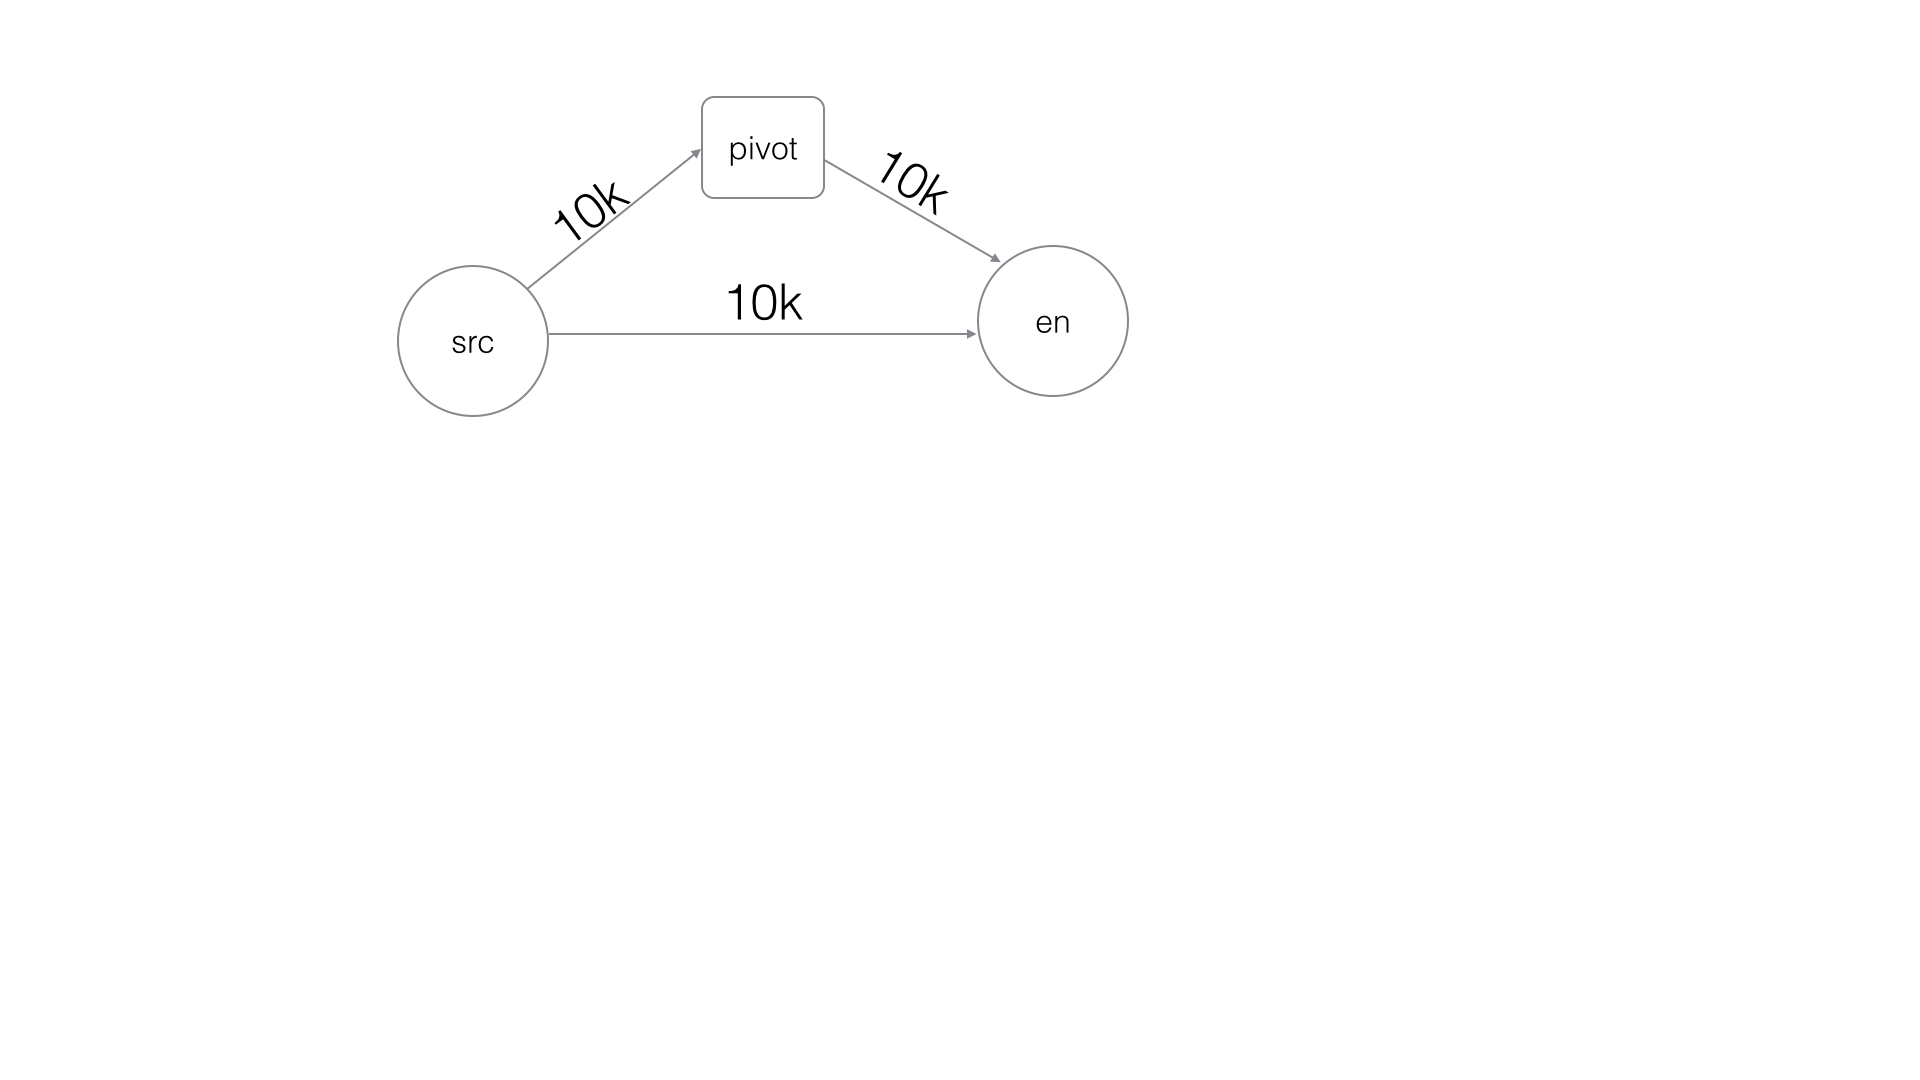
\includegraphics[scale=0.2]{files/Figures/Cohn.jpg} \\
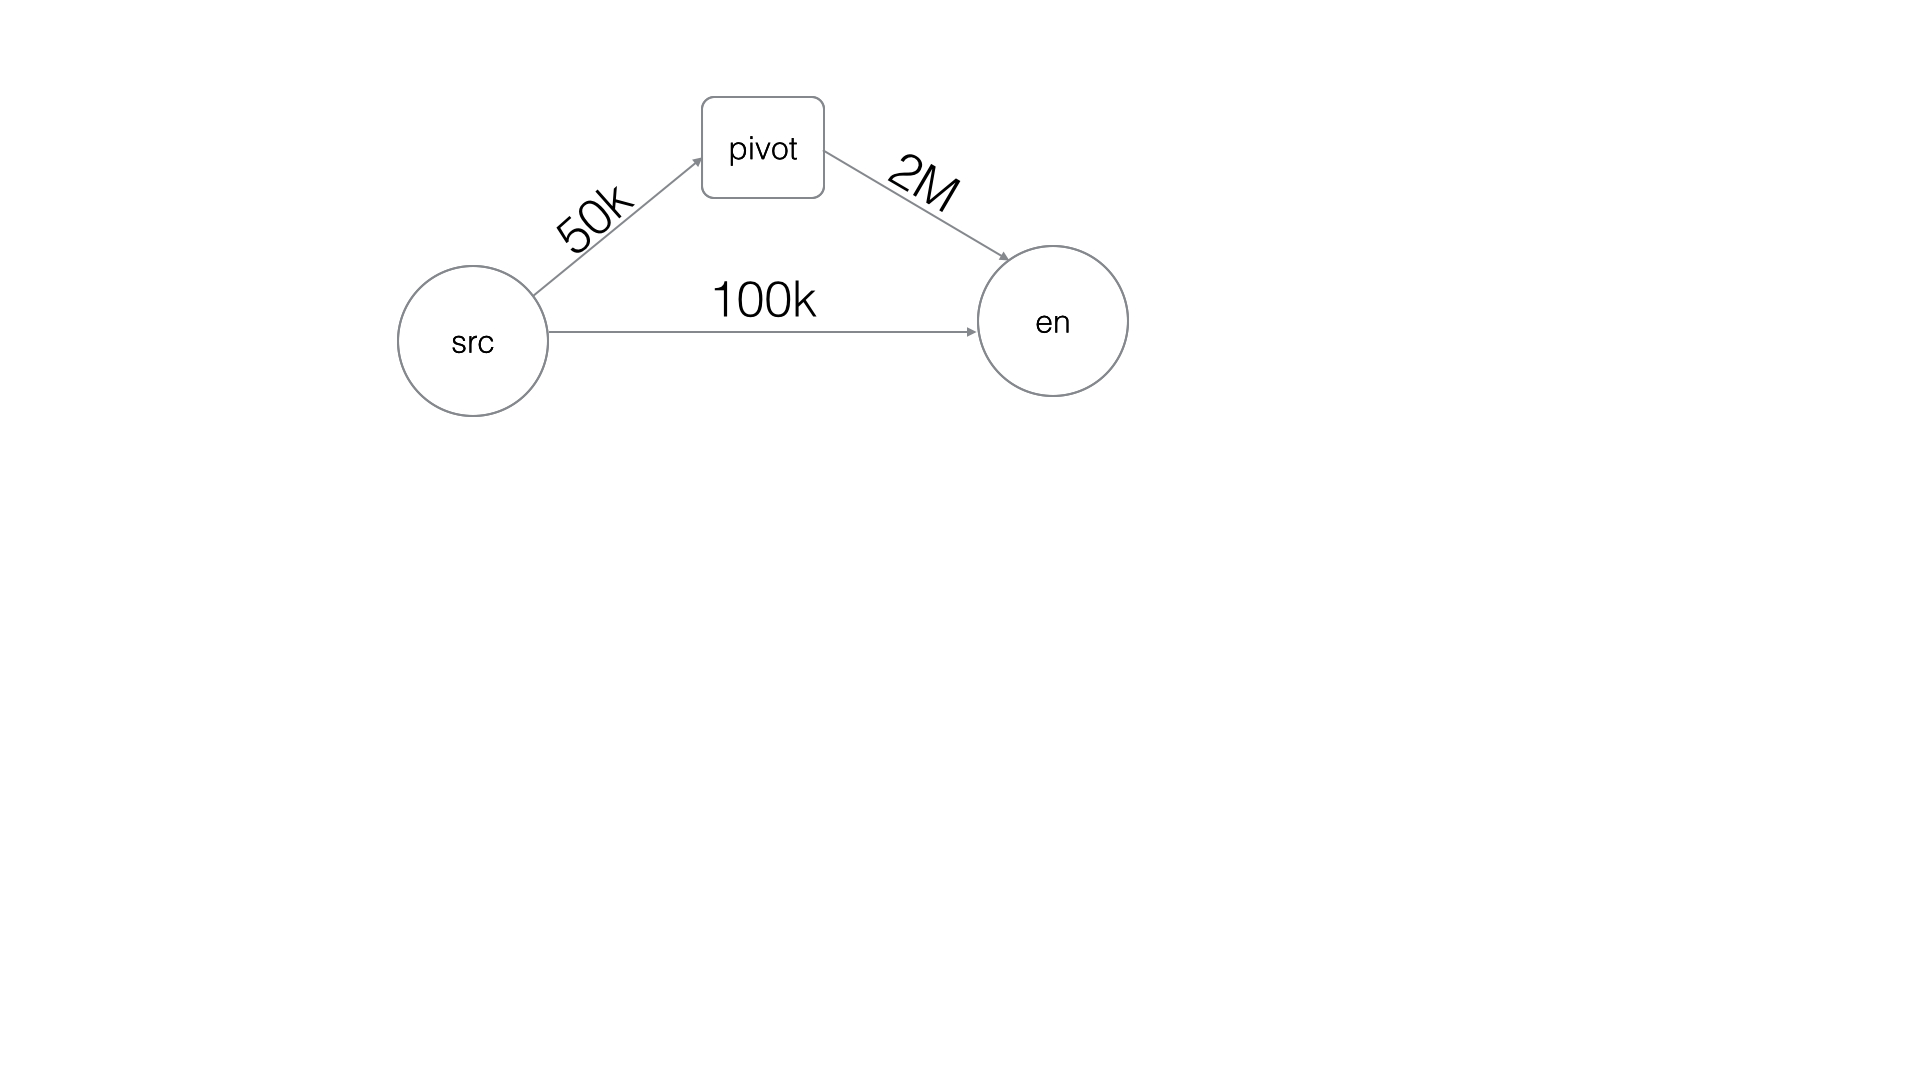
\includegraphics[scale=0.2]{files/Figures/Our.jpg} \\

\section{Experiments}
\begin{tabular}{lr}

\toprule
System & BLEU \\
\toprule
es-en & 23.32 \\
fr-en & 19.53 \\
de-en & 15.60 \\
\bottomrule
\centering
\small
\label{table:eparl100}
\end{tabular} \\
\begin{tabular}{lrrrrrr}
\toprule

src-tgt & pivot & top20 & top40 & top60 & top80 & top100 \\
\toprule

de-en & fr & 13.32 & 13.33 & 13.35 & 13.42 & 13.03 \\
de-en & es & 13.37 & 13.17 & 13.49 & 13.34 & 13.36 \\
fr-en & de & 16.21 & 15.82 & 15.89 & 16.08 & - \\
fr-en & es & 17.77 & 18.15 & 17.99 & 18.01 & 18.27 \\
es-en & fr & 21.35 & 21.18 & 20.83 & 21.01 & 21.45\\
es-en & de & 18.36 & 19.19 & 19.35 & 19.23 & 18.97 \\
\bottomrule
\centering 
\small
\label{table:eparltopn}
\end{tabular}
 \\

\section{Remarks}










%!TEX root=/home/ska124/Dropbox/Thesis/thes-full.tex

%%%%%%%%%%%%%%%%%%%%%%%%%%%%%%%%%%%%%%%%%%%%%%%%%
%
%     Chapter 6
%
%%%%%%%%%%%%%%%%%%%%%%%%%%%%%%%%%%%%%%%%%%%%%%%%

\chapter{Conclusion}
\label{chap:conclusions}

\section{Summary}
\label{sec:summary}

\section{Paying it forward}
\label{sec:pay_it_forward}





%%%  appendices, if any
% \begin{appendices}
% %!TEX root=/home/ska124/Dropbox/Thesis/thes-full.tex
%% Copyright 1998 Pepe Kubon
%%
%% `appone.tex' --- 1st appendix for thes-full.tex, thes-short-tex from
%%                  the `csthesis' bundle
%%
%% You are allowed to distribute this file together with all files
%% mentioned in READ.ME.
%%
%% You are not allowed to modify its contents.
%%

%%%%%%%%%%%%%%%%%%%%%%%%%%%%%%%%%%%%%%%%%%%%%%%%%
%
%        Appendix 1
%
%%%%%%%%%%%%%%%%%%%%%%%%%%%%%%%%%%%%%%%%%%%%%%%%

% \chapter{}
\label{app:spacing}


% %!TEX root=/home/ska124/Dropbox/Thesis/thes-full.tex
%% Copyright 1998 Pepe Kubon
%%
%% `apptwo.tex' --- 2nd appendix for thes-full.tex from
%%                  the `csthesis' bundle
%%
%% You are allowed to distribute this file together with all files
%% mentioned in READ.ME.
%%
%% You are not allowed to modify its contents.
%%

%%%%%%%%%%%%%%%%%%%%%%%%%%%%%%%%%%%%%%%%%%%%%%%%%
%
%        Appendix 2
%
%%%%%%%%%%%%%%%%%%%%%%%%%%%%%%%%%%%%%%%%%%%%%%%%

\chapter{Illustrating Lists}\label{app:lists}
\index{formatting of Lists}

This appendix is present only in the full version of the thesis. It
illustrates in more detail the formatting of the Lists of Tables,%
\index{List of Tables}\index{List of Figures} Figures, etc. In
addition, it also illustrates the use of the ``other list'' facility
of \textsf{csthesis.sty}\index{csthesis.sty@\textsf{csthesis.sty}}.
Let us start with the latter.

\section{List of Programs}
\index{List of Programs}

In the preamble of \texttt{thes-full.tex}%
\index{thes-full.tex@\texttt{thes-full.tex}}, a new type of a floating
environment---\texttt{program}%
\index{program environment@\texttt{program} environment}---is defined,
together with the \verb+\otherlist+%
\index{otherlist@\texttt{\symbol{'134}otherlist}} command for
typesetting the List of Programs. The list is formatted in the same
way as the lists of Figures and Tables, and an appropriate entry is
added into Contents.

Because programs are defined here as floating environments, they are
typeset with the same (tighter) line-spacing%
\index{spacing in programs} as figures and tables:

\begin{program}[htbp]
  \begin{center}
    This shows that single line spacing\\
    is used inside programs.
    \caption{Example of the new \texttt{program} environment\label{prog1}}
  \end{center}
\end{program}
%
\vspace*{-.3in}
\begin{program}[htbp]
  \begin{center}
    A second example of a program environment.
    \caption{Second program\label{prog2}}
  \end{center}
\end{program}

\section{Formatting of Lists}

The tables (figures, programs, etc.) are organized and sorted by
chapters (appendices), with additional small vertical space separating
the chapter blocks. To illustrate this, I include two new tables here
(see List of Tables, etc., in the beginning of the thesis for the
result)\index{formatting of Lists}:

\begin{table}[htbp]
  \begin{center}
    To be silly or not to be silly\\
    \emph{that} is the question!
    \caption{First meaningless table in Appendix~\ref{app:lists}}
  \end{center}
\end{table}
%
\vspace*{-.3in}
\begin{table}[htbp]
  \begin{center}
    $F = nd^{2}$
    \caption{Second meaningless table in Appendix~\ref{app:lists}}
  \end{center}
\end{table}


% \end{appendices}

%%%%%%  bibliography
%!TEX root=/home/ska124/Dropbox/Thesis/thes-full.tex
%% Copyright 1998 Pepe Kubon
%%
%% `bibl.tex' --- bibliography for thes-full.tex, thes-short-tex from
%%                the `csthesis' bundle
%%
%% You are allowed to distribute this file together with all files
%% mentioned in READ.ME.
%%
%% You are not allowed to modify its contents.
%%

%%%%%%%%%%%%%%%%%%%%%%%%%%%%%%%%%%%%%%%%%%%%%%%%
%
%       Bibliography
%
%%%%%%%%%%%%%%%%%%%%%%%%%%%%%%%%%%%%%%%%%%%%%%%%

\nocite{*}     % everything cited automatically

\renewcommand{\baselinestretch}{\tighttextstretch} %% get smaller spacing
\normalsize

\bibliographystyle{plain}   %% dash under repeated name, von ignored
\addcontentsline{toc}{chapter}{Bibliography}
\typeout{Bibliography}
\bibliography{files/thes-both}
\renewcommand{\baselinestretch}{\textstretch} %% get normal spacing
\normalsize



%%%%%%  index
% %!TEX root=/home/ska124/Dropbox/Thesis/thes-full.tex
%% Copyright 1998 Pepe Kubon
%%
%% `ind.tex' --- index for thes-full.tex from
%%               the `csthesis' bundle
%%
%% You are allowed to distribute this file together with all files
%% mentioned in READ.ME.
%%
%% You are not allowed to modify its contents.
%%

%%%%%%%%%%%%%%%%%%%%%%%%%%%%%%%%%%%%%%%%%%%%%%%%
%
%       Index
%
%%%%%%%%%%%%%%%%%%%%%%%%%%%%%%%%%%%%%%%%%%%%%%%%

\renewcommand{\baselinestretch}{\tighttextstretch} %% get smaller spacing
\normalsize

\addcontentsline{toc}{chapter}{Index}
\typeout{Index}
\printindex

\renewcommand{\baselinestretch}{\textstretch} %% get normal spacing
\normalsize



\end{document}

